\documentclass[12pt]{report}

\usepackage[utf8]{inputenc}
\usepackage{blindtext}
\usepackage{amsmath}
\usepackage[margin=2cm]{geometry} 
\usepackage{graphicx,changepage}
\usepackage{xcolor}
\usepackage{hyperref}
\usepackage{tcolorbox}
\usepackage{subfig}
\usepackage{fancyvrb}
\usepackage{listings}
\usepackage{dirtytalk}
\usepackage{csvsimple}
\usepackage{float}
\newcommand\todo[1]{\textcolor{red}{#1}}
\title{The Legend of Bluespec: A Link to the components}
\author{kr469 }
\date{October 2021}
 \hypersetup{ 
     colorlinks=true, 
     linkcolor=cyan, 
     filecolor=cyan, 
     citecolor = black,       
     urlcolor=cyan, 
     } 
\tcbset{colback=pink!7,colframe=pink!90,coltitle=black}
\begin{document}
\maketitle
\tableofcontents

\chapter{Introduction}
Making hardware is hard, and similarly to other problems in computer science, we make it easier by adding layers of abstraction. There are many layers, diagram below shoes simplified overview of them. The layer this project focuses on is going from modules to integrated systems. At this layer, we already have code for modules like memory, CPU cores, interconnects etc. There we need an ability to compose them in such a way that they create a whole device. My project will focus on doing that.
\begin{figure}[h!]
    \centering
    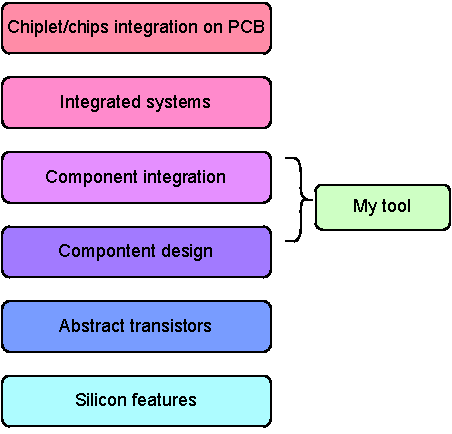
\includegraphics[width=0.5\columnwidth]{pdfExports/LargeMapLayersOfAbstraction.pdf}
    \caption{Stage one of node used to instantiate new modules}
\end{figure}
% \begin{figure}[!h]
%     \centering
%     \caption{Layers of abstraction when designing hardware}
%     \includesvg[width=0.7\columnwidth,path=svgExports]{layers.svg}
% \end{figure}
\section{Motivation}
\begin{tcolorbox}[title=Vocabulary]
    \begin{itemize}
        \item Verilog - Hardware description language
        \item Bluespec - Hardware description language
        \item Intel Quartus Prime (IQP) - programmable logic device design software produced by Intel. (source \href{https://en.wikipedia.org/wiki/Intel_Quartus_Prime}{Wikipedia})
        \item Platform Designer - Tool inside IQP used to connect high level components.
    \end{itemize}
\end{tcolorbox}
Verilog is an old language with a minimal type system. It forces people to encode more complex interfaces using finicky naming conventions. To simplify the process of connecting components with many wires, people tend to use high-level tools like Platform Designer, which has built-in logic allowing for easy connection of components. This approach is not perfect and as we will see during the evaluation, a better option might be to move away from Verilog and use a more modern language like Bluespec. Bluespec's type system allows us to detect connectable things in a systematic manner and allows us to define how to connect them. In fact large body of Bluespec modules are already defined in this manner. Currently, there are no tools for automated system composition for native Bluespec modules. If we want to do this high level integration Bluespec components then we need to transpile Bluespec code into Verilog to make then importable to tools like IQP. Unfortunately, because of typing richness of Bluespec (comparable to Haskell), arbitrary code cannot be transpiled, and before code can be transpiled, it needs to be stripped of any arguments or other kinds of polymorphism. This process of transpilation also destroys high-level interfaces, and they must be recreated manually after importing Verilog code into IQP.

\section{Already existing tools}
During evaluation of this I will compare my tool with Platform designer from IQP. 
Platform Designer is a GUI tool for high-level integration, designs generated by it are kept in verbose text file format. Unfortunately, those files tend to be megabytes long for larger projects, making them hard to read and edit, for humans. 
There are other problems with using Platform Designer, like the cumbersomeness of importing new components.

\begin{tcolorbox}[title=Market share and justification for focusing entirely on comparisons with Intel Quartus Prime]
    It is a bit difficult to accurately judge the market share of IQP, but It is produced by one of the biggest designers and manufacturers in the world, and it is also used by Qualcomm according to \href{https://discovery.hgdata.com/product/intel-quartus-prime}{HG Insights}. Using Google trends we can see that in recent years (since 2016) competitor Xilinx Vivado has overtaken IQP in interest at the global scale, in most developed countries like the US, Europe, and parts of Asia. There is roughly 50/50 split between IQP and Vivado. My personal observations suggest that Xilinx Vivado became highly popular in India which is a large country with a history of chip design, and this might be strongly skewing data in favour of Xilinx's product. I chose to compare against IQP because we learned to use it in our course.
\end{tcolorbox}

\section{Proposed solution}
During my project, I created a system for finding connectable things and supplying some other data for high level GUI applications. There are two main ways of interacting with this system. First one using JSON files describing systems. Those JSONs are simpler and more human-readable, than comparable files used by IQP. 

Reading of such JSONs is rather unimpressive on its own, and one might argue that it would be better to use Bluespec code instead of it. The interesting part of this project lies in the backend that can verify correctness of this file and produce a set of typing information about produced Bluespec code.  

But to truly appreciate the work I have done during this project, I also implemented GUI, which uses the same backend as the one used to interpret JSON files and is able to supply the user with typing information and possible choices when connecting components.  

One can think of it as a Bluespec native high-level integration tool that uses a simple language server in the backend. This way Bluespec users can do high-level integration in the domain of not transpiled Bluespec code. Then after a satisfactory top-level module is created, it can be transpiled to Verilog and then imported into IQP. 

\chapter{Preparation}
This section will give you basic understanding of concepts found in Bluespec (most importantly provisos and typeclasses). It will explain language I used. Finally, it will talk about grammar needed to parse information about types.
\section{Understanding Bluespec}
Before I started this project, my only knowledge about Bluespec came from \href{https://www-bluespec.cl.cam.ac.uk/}{Cambridge Bluespec Tutor} which covers basics, and it was completed by me a few weeks before the start of this project. To understand this project, I have learned about most of the type system of Bluespec, but for you, the reader, most of it is not relevant. Therefore, I prepared a short tour of things that will be important to understand in this project. 
\subsection{Rules}
In Bluespec all computation is done in form of rules.  
Each cycle we will take a subset of all rules that we are going to execute in this cycle. The rule is fired (executed) in the cycle only if it is ready (or will be ready) and it is not conflicting with other rules (If this happens compiler must issue a warning and picks an arbitrary rule to fire from a subset of conflicting rules). Each rule can fire at most one-time per cycle.  
For a rule to be ready to fire, it needs its implicit and explicit conditions to be true.  
A rule can be fired in a cycle even if it is not ready at the start of a cycle, for example, if you add an item to an empty queue and then pop can happen in the same cycle. \\ 
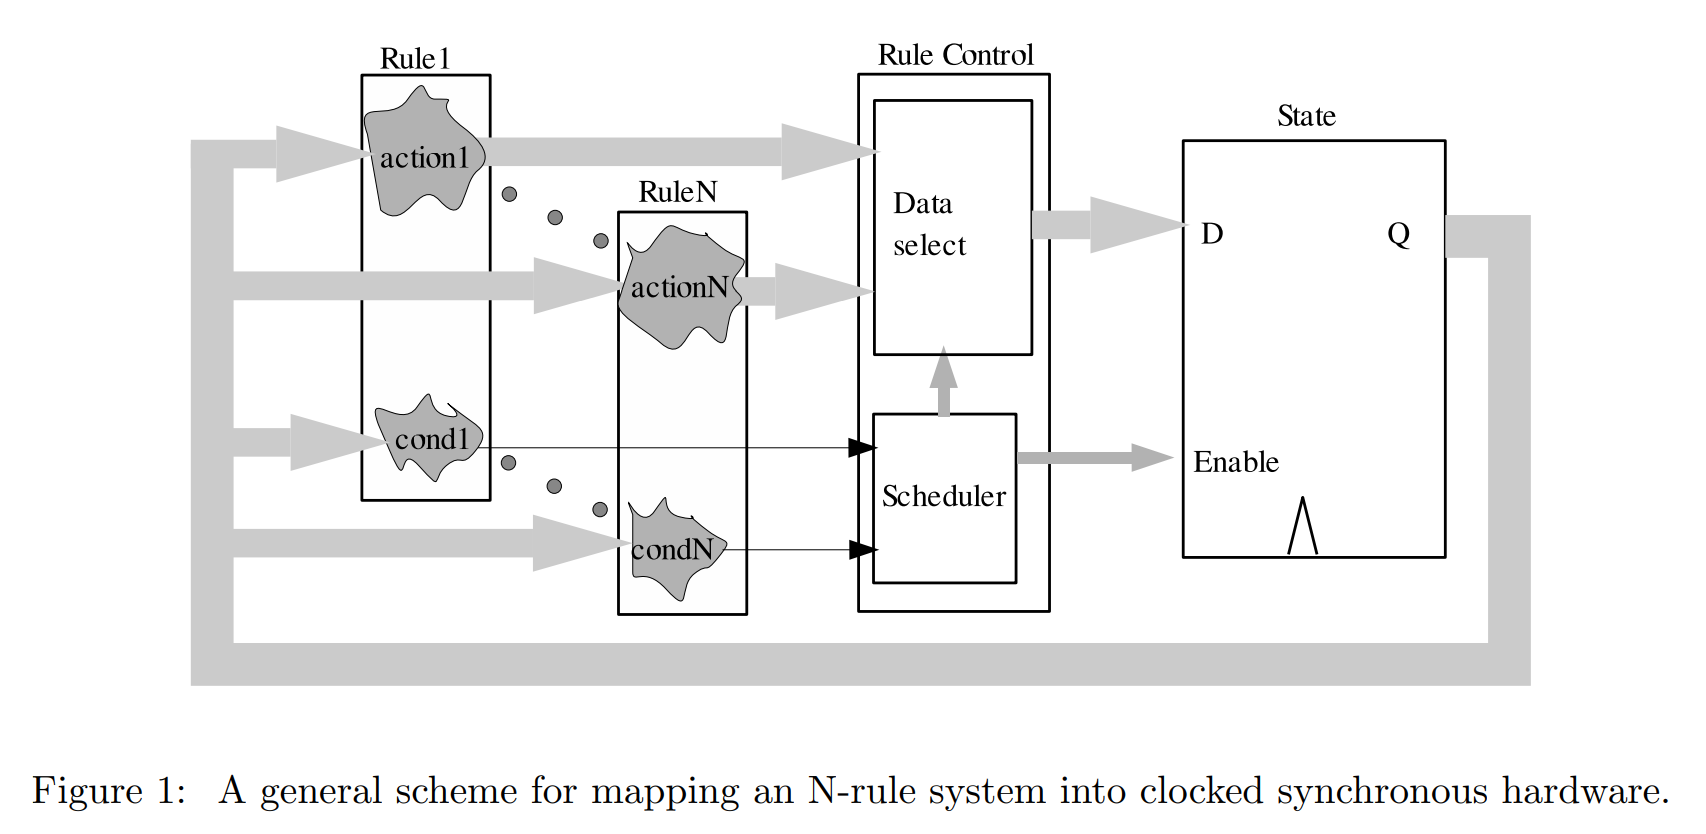
\includegraphics[width=\textwidth]{Rulemapping.png} 
(TODO: add a reference to the bsv reference document from which this image was taken) 
\begin{verbatim} 
        
   TODO: a piece of Bluespec with the module using FIFO and another rule 
    explaining types of conditions. 
    
\end{verbatim} 

\subsection{Modules and interfaces}
Module is unit of organization of logic. Modules don't have types, instead they implement some interface. This means that you can have multiple modules with different behaviour that implement the same interface. It might be helpful to think about similarly to different physical connectors(like USB-C, PCI-e). Interfaces are made up out of two types of things:
\begin{itemize}
    \item Methods - that allow for interaction with the module, they come with few variants, but this is not important for now.
    \item Subinterfaces - That allow for more generalization, for example if you want to implement module that contains two copies of the same interface, you can just create a new interface that contains two instances of that subinterface and assign them accordingly.
\end{itemize}

\subsection{Typeclasses}
\label{sec:Typeclasses}
Typesclasses in Bluespec are used to group types for which specific functions or modules are implemented. Typeclass instance is (TODO describe what is it) and it can have provisos attached to it.

\subsection{Provisos}
\label{sec:Provisos}
One big feature of Bluespec typing is support for provisos. They create constraints on types that can be used with a given function and give information about the expected type of the output of the function during compilation. For example, we can have a polymorphic function \verb!extend! of a type \verb!Bit#(a)! $\rightarrow$ \verb!Bit#(b)! where \verb!Bit#(x)! is a vector of $x$ bits, such function accepts vector any length $a$ and always return vector of length $b=a+1$. To make sure these relations stay like this, we would attach a proviso \verb!Add#(a,1,b)! which means that $a+1$ must be equal to $b$.  
\par  
Mentioned above \verb!Add! is one of the Size Relationship provisos, other such provisos are \verb!Mul! \verb!Div! \verb!Max! \verb!Min! \verb!Log!.  
Those provisos cannot be nested, but we still can express complex arithmetic constraints, thanks to size relationship type functions.  
They essentially represent the result of the operation on values that were supplied. There are only 8 of them, and they are \verb!TAdd! \verb!TSub! \verb!TDiv! \verb!TMul! \verb!TMax! \verb!TMin! \verb!TLog! \verb!TExp!.  
To better explain this, let us look at this simple example: \\  
\verb!Add#(TExp#(a),TDiv#(a,8),c)! is a proviso that says that the following equation $2^a+\lceil\frac{a}{8}\rceil = c$ on parameters \verb!a!,\verb!b!,\verb!c! must be satisfied. Otherwise, it will mean that supplied parameters are not valid and compilation won't succeed. Those equations can be also solved to deduce unknown parameters.  
\par  
There is also another type of provisos that I will call \emph{typeclass based} ones.  
Typeclass based provisos allow us to either ensure certain functions are defined for a given type or to deduce something. For example, \verb!Bits#(a,b)! means that for type \verb!a!, there must be functions \verb!pack! and \verb!unpack! allowing for convertion to and from a vector of $b$ bits. Moreover, this can be used to get the length in bits of given objects, on which we can later put constraints using Size Relationship provisos.  
In my project, I will often check if there exists an instance of the \verb!Connectable#(a,b)! typeclass for a given pair of types \verb!a! and \verb!b! to check if function \verb!mkConnection! (used to connect two interfaces together) is defined.  
All of this can be a bit confusing, but if one looks closely, system of provisos and typeclasses is remarkably similar to Prolog the programming language. We have variables that are effectively the same as in Prolog, we have values that are integers, and we have parametric types and functions that are like Prolog's compound terms. Typeclass are like groups of rules with the same name, and provisos attached to Typeclass instances are like predicates attached to rules.  

One significant difference is that provisos can be solved in arbitrary order, which means that unlike in the Prolog, we need the ability to solve sets of equations on integers to resolve them.

\section{Choosing tools}
I had effectively 3 choices for a language to write this project in. Here is some justification for why I have chosen Python.   

\subsection{Haskell}  

The compiler of Bluespec is written in Haskell. Therefore, there are several reasons why Haskell would be the right choice. Here are some of them:  
\begin{itemize}  
   \item I can reuse already written logic.  
   \item I will not diverge in terms of logic from Bluespec compiler.  
   \item I will not need to write grammar to load packages.  
\end{itemize}  
But there are also a few particularly good reasons why I did not use Haskell.  
\begin{itemize}  

   \item I never used Haskell before, and my experience with functional languages is equal to what was shown in the foundations of the computer science course.  

   \item I never used Bluespec before, and my experience is limited to completing the Bluespec tutor provided by the computer science department.  

   \item Even if I knew Haskell and Bluespec, industrial compilers are rather large and complicated. I also received advice to avoid modifying/extending them as a part of the project.  

\end{itemize}  

While each of those reasons on its own is something that can be managed. All of them combined would create an unacceptable amount of risk of not delivering the project. There was also a chance that the use of Haskell would not create a good story for the project. (This is quite subtle). 

\subsection{Tcl (pronounced "tickle")}
This language is used as a scripting language in both Intel and Xilinx tools, While I will be reading packages using Tcl scripts provided by the creators of the Bluespec compiler (BSC), my understanding is that those scripts are just handy wrappers for some Haskell functions. This is also a foreign language to me, with a minimal presence online and negligible learning resources, making it difficult to learn. It is also quite obsolete, and there is not much tooling for it making it undesirable as a time investment (As an example of the desirable to learn technology. I learned for this project JavaScript just to create a GUI). 
\subsection{Python}
Firstly, this is a language I have experience working with. Secondly, it is widely supported, and there is extensive tooling for it. Its flexible typing system allows for rapid experimenting, which was especially handy when I was not sure what the structure of the data would look like. It is also worth mentioning that Python has support for typing, and at some point, I decided to start adding typing hints around. My rule of thumb that I used was that if Pylance (Python language server) cannot deduce the type of something, I need more hints.  
Other reasons for using Python are:  
\begin{itemize}  
  \item I will have many interesting problems to solve. Like creating and interpreting grammar.  
  \item Code written in it can be used by a large community of python developers.  
  \item I can use many tools like Lark (for grammar), Django (as a backend server), and SymPy (to solve size relationship provisos) that will speed up the process.  
\end{itemize}  
The two arguments against using Python are:  
\begin{itemize}  
  \item Haskell would be better suited for this task. I explained above why it does not make sense for me to use Haskell.  
  \item Python is usually slow. Fortunately, this is not a big issue thanks to caching and the use of PyPy (implementation of Python using JIT compiler).  
\end{itemize} 
\subsection{Postmortem}
Looking at those choices now (after finishing the project and knowing all encountered difficulties), I could have also considered \verb!C#!, due to its speed and similar typing flexibility to Python. I also think Haskell would be a better choice if this were more like my pet project on which I would work for a few years to make it a commercially viable product.  
  
\section{Creating a grammar}  
This section could be moved into implementation.  
  
\begin{tcolorbox}[title=Bluetcl]  
  Bluetcl is a tool written in Tcl language that allows for inspection of Bluespec packages. It is a first-party tool that is included with the Bluespec compiler. There is not much documentation about it, but from my understanding, it is a wrapper around Haskell's code.  
  From the user perspective, it is just a bash script that starts the Tcl terminal compiled with some libraries. From my perspective, I use it as an arbitrary command-line program, as this method of use is intended by the authors and contains some documentation.  
\end{tcolorbox} 
\subsection{What grammar is needed ?}
Because I am using Bluetcl as a command-line tool, communication with it is done via text.  
While synthesizing commands is easy, parsing outputs is a bit more difficult, and I decided to do it systematically.  
To do this, I need the grammar of all possible outputs that I am interested in.  
Bluetcl produces a range of outputs, but two of them that are particularly useful are descriptions of functions and descriptions of types.  
\subsection{Where to find this grammar?}  
Unfortunately, this grammar is not documented anywhere, so I had to reverse engineer it. This approach might not be perfect and might not cover every input, but it is good enough to parse every standard package and all packages used to compile Flute (RISC-V CPU with 5 stage pipeline).  
Here are other reasons to justify this approach:  
\begin{itemize}  
   \item Heaps' law suggests that the number of unique words in a given body of the text is proportional to approximately the square root of the number of words in the text. Therefore, it is fair to assume that something similar will be true if we consider the number of unique grammar rules.  
   \item This grammar, while different from the grammar of Bluespec the language maps a subset of Bluespec grammar, so we can supplement our deductions with a reference guide for Bluespec language. Therefore, accounting for cases we have not seen, but are possible.  
   \item There are also some limitations on how exotic things can get in top modules. (TODO rephrase this)  
\end{itemize}

\subsection{Technical aspects of the grammar}
This is EBNF grammar, I parse it using Lark library for Python, and I am using Earley parser, as it is capable of arbitrary length lookahead. The grammar I created contains roughly 90 rules, and I will not include all of them here, but I will show an example to give a feel of what is happening. (TODO: Think about dumping them into an appendix)   
\\   
A useful feature supported by Lark is the ability to have regular expressions in the grammar. I am mentioning this as it is effectively like having a parser inside a parser. It is also worth mentioning that there exists a handy tool for debugging and creating grammar. It is located at this website: \href{https://www.lark-parser.org/ide/}{https://www.lark-parser.org/ide/} and it can run the parser online and show created AST tree. 
\begin{tcolorbox}[title = Parsing position TODO maybe find a better example with shorter line]
Here is an example of parsing a small section of output that describes the location of a piece of code that is being described. I decided to show it as it's simple and shows different features that I needed to use.
    \begin{verbatim}
-------- Rules used ------------
identifier_u: /[A-Z][\w$_']*/

tcl_position: "{" "position" "{" tcl_path NUMBER NUMBER 
 ["{" "Library" identifier_u "}" ]"}""}"

tcl_path: ["%/"] /((\.{1,2})|(\w|-|\s)+)/ 
 ["/" /((\.\.)|(\.)|((\w|-|\s)+))/]* "." /\w+/

-------- Text to parse ---------
{position {%/Libraries/Connectable.bs 25 1 {Library Connectable}}}
    \end{verbatim}
    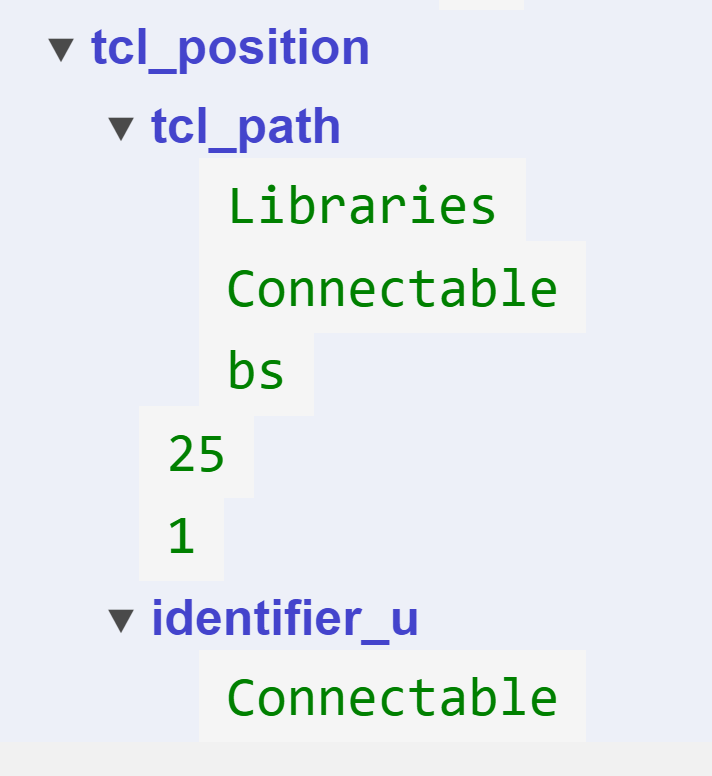
\includegraphics[width=0.4\textwidth]{images/TCLPath.png}
\end{tcolorbox}


\chapter{Implementation}
Before I will explain how top modules are built, I will explain first how Bluespec packages are crawled to extract typing information as it is essential for building top level module. 
\section{Crawling the packages}
\begin{figure}[!h]
    \centering
    \caption{Overview of process of crawling packages}

    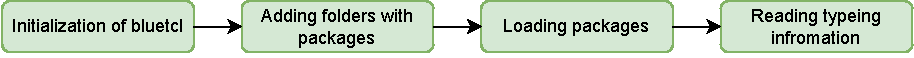
\includegraphics[width=1.0\columnwidth]{pdfExports/LargeMap-Crawling.drawio.pdf}
\end{figure}
To interact with Bluetcl, I have written a script using the Pexpect library. This script works by creating a subprocess of Bluetcl and exposes functions that allow for the performing of quarries. The core of this script is a function called \verb!call! that takes as input a string that is a command and returns the output of stripped of warnings or raises an exception if an error occurred (for example: in the case where a package was not found). To remove warnings, I make some assumptions. 
\begin{itemize}
    \item I only use a fixed set of commands (like list packages, describe a type).  
    \item For those commands important output is always on the last line. (This was checked empirically)   
    \item Output of command is always followed by $\%$ a character that never occurs in the rest of the output and marks the end of the output.  
\end{itemize}   
Thanks to them, I do not need a sophisticated system for parsing errors and or warnings. I can just make a quick search for the error, and if needed forward this to the user.  
  \\   
In total, this script allows me to:   
\begin{itemize}   
\item Initialize subprocess   
\item Add folder to search path of Bluetcl   
\item Load package (Bluetcl takes care of finding and loading dependencies)   
\item Get the list of loaded packages   
\item List functions in a package   
\item List types in a package   
\item Get information about types and functions in the package   
\end{itemize} 

\section{Loading Bluespec packages' information (TODO check grammar of s')}  

\begin{figure}[!h]  
   \centering  
   \caption{Overview of parsing bluetcl data}  
   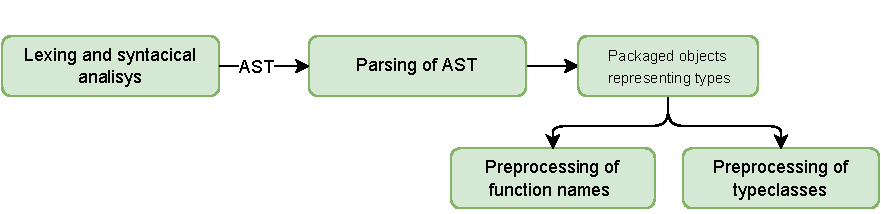
\includegraphics[width=1.0\columnwidth]{pdfExports/LargeMapProcessing.pdf}  
\end{figure}  

As mentioned earlier output of bluetcl is text, and I need it in some better-organized form. In this section, I describe the process of doing this.  
\subsection{Lexical and syntactic analysis}  
I decided to use the Lark library for lexical and syntactic analysis. This library takes grammar and strings of text as input and returns an abstract syntax tree. The only difficult part here is creating grammar, but we have taken care of it during preparation. (TODO improve this last sentence)  
\subsection{Understanding abstract syntax tree (AST)}  

Given AST I needed to turn it into a more useful form. To do this I used \verb!Transformer! the class provided by Lark. The way it worked is that I created a subclass of \verb!Transformer! that implemented a function for each non-terminal / rule(Each non-terminal can have multiple rules and Lark allows for renaming of individual rules, for example, this allows parsing different non-terminals using the same function or parsing single non-terminal using different functions depending on rule that was used). \verb!Transformer! will then perform a bottom-up transformation of AST, and for each rule, it will call the respective member function, with parsed children (non-terminals used by rule) as arguments. At the end of the transforming process, I have a list of objects that represent data from Blutecl.  
\par
One of the bigger inconveniences I encounter is the fact that Lark passes parsed children, as a simple list. This does not provide information about what exactly each child is, this is not a problem if the rule contains a fixed number of non-terminals, but otherwise, I employ a mix of length-based inference, and wrapping of data from children into tuples, to provide remove ambiguity.  
\par
What was quite useful at this stage is Python's type system flexibility, I was able to gradually build up \verb!Transformer! class and add typing information only after I had a firm understanding of what type something needs to be. For some things, it was not immediately obvious what is the best way to represent them, and what often happens is I would first leave them as lists of unparsed things. Then after I got to the point where I needed to use them, I would decide what is an optimal way to represent them. 

\subsection{Organizing data and functionality}
I created a class called \verb!TypeDatabase! that provides set of functions that manage loading packages and parsing packages' information. It is also capable of loading and storing previously stashed state from a \say{pickle} file. This saves a lot of time as parsing and communication with bluetcl isn't particularly fast. This class is also a home to set of functionality used to resolve types. From my testing it takes about 370s to load roughly 250 packages that I found included with Bluespec compiler and created to compile Flute CPU. Loading those packages from cached files takes 5 to 20 seconds.

\newpage
\section{Building the top level module}
\begin{figure}[!h]
    \centering
    \caption{Overview of the flow of data in the top level module}

    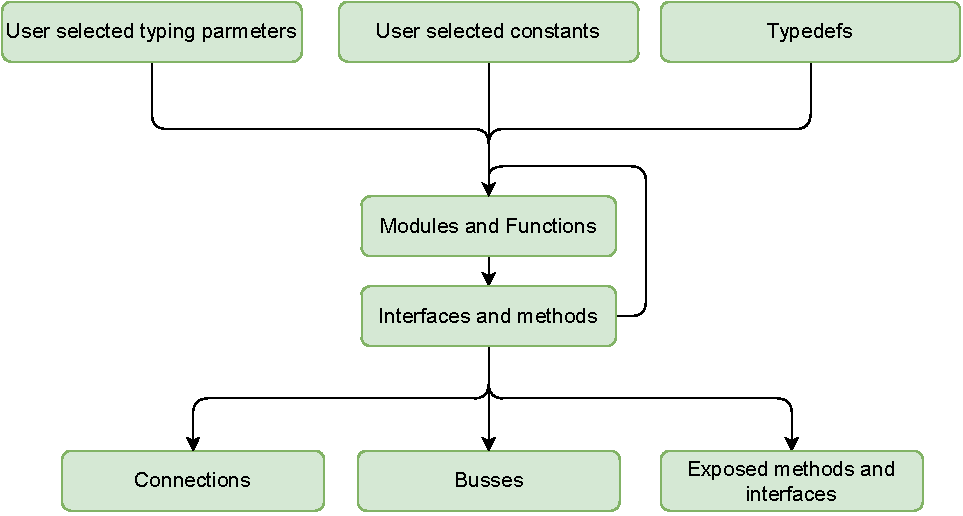
\includegraphics[width=1.0\columnwidth]{pdfExports/LargeMap-dataFlow.drawio.pdf}
\end{figure}
The above diagram shows the flow of data during the creation of the top-level module. Users can specify all nodes of this diagram with exception of \emph{Interfaces and methods} produced by \emph{Modules and functions} as this is specified by typing information. 
Building the top-level module can be broken down into a few operations. 
\begin{itemize} 
   \item Instantiating new modules. 
   \item Connecting modules using \verb!mkConnection! function. 
   \item Connecting modules using busses, using functions of certain characteristics. 
   \item Specifying exported interfaces and methods. 
\end{itemize}  
Operations of Instantiating new modules, Connecting and Creation of Busses are quite similar, so I will start by describing Instantiating new modules and then how it fits with other operations. 
\subsection{Instantiating new modules} 
To instantiate the new module, we need to do the following things: 
\begin{enumerate} 
   \item Convert inputted by user strings to type identifiers. This includes converting the names of interfaces and their members to their type identifiers. 
   \item Checking if arguments provided are of valid types. 
   \item Checking if typing information satisfies provisos. 
   \item Add newly created interfaces and methods to the namespace of known names. 
\end{enumerate} 
From this list items, 1 and 4 are implemented using a few dictionaries that keep track of known names and their types. I also have a system that keeps track of which instantiated things depend on which other instantiated things. Thanks to this system, I am able to create a graph of dependencies, which is used to order things in the right order. As for things mentioned points 2,3, they are compleated using later described functions for type resolution. 
\subsection{Connections}
Adding a new connection is easy, as this can be done using the same logic as \emph{instantiating new modules}. What is more interesting is that I keep track of all possible connections that can be made. This is later used to supply autocompletion in GUI (If the user uses JSON based interface, I can just print this data). Tracking of those connections is done in a naive way by simply checking all possible $O(n^2)$ connections. A question that arises is: "Can I do better?". While I do not have concrete proof of this, execution of program written in Prolog can be reduced quite nicely to checking whether two types are connectable. Therefore whole problem of finding all pairs of connectable things can be reduced to the following problem.
\par
Given $n$ \emph{input values} (number of interfaces and methods in instantiated modules) and $k$ input \emph{programs} (number of instances of typeclass \verb!Connectable!) find all pairs of two \emph{input values} for which at least one \emph{program} halts with the resulting value being true.
Unfortunately, Prolog is a touring complete language, and it's hard to do much better than naive brute force.
This sounds like a lot of work, but thanks to look-up dictionaries, usually I need to check only a few \emph{programs}. I also spread out the work over subsequent additions of new modules and did not recompute already known results. This way, the user will perceive lag roughly proportional to the number of modules already instantiated. I also noticed that with a larger number of modules, PyPy's JIT compiler will step in, and it will produce more optimized code, therefore keeping computation time low. 
 
\subsection{Busses}
When it comes to busses, most logic goes to synthesizing code for them, and not figuring out whether given data is valid, because of this I can fall back on logic designed to instantiate modules. To synthesize a bus, I need to synthesize a routing function.
A routing function is a function that takes a route and produces a one-hot vector that specifies which slave is used for a given address. 
To create a routing function, two things must be created. First, I need to create a new function and add it to the database of known functions. To do this, I just reuse my parsing tooling. As for creating code for it, I generate a user template and fill it with \verb!if! statements for each address region(I don't need to do fancier logic as in hardware, it will be optimized anyway). I also generate comments giving information about which slaves occupy which address region.

\subsection{Specifying exported interfaces and methods}
This functionality utilizes data generated previously, and most logic behind it focuses on supporting a few special cases that are meant to keep produced code clean.

\section{Resolving types}
\begin{figure}[!h]
    \centering
    \caption{Dependencies between functions}

    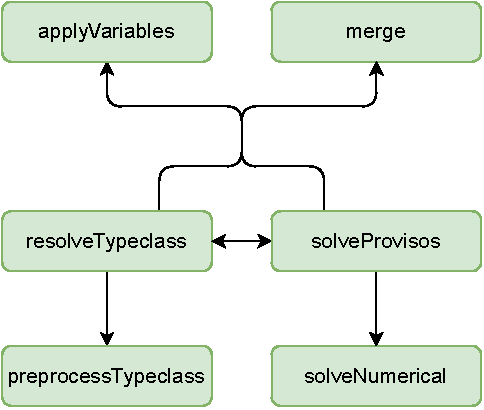
\includegraphics[width=0.5\columnwidth]{pdfExports/LargeMapResolve.pdf}
\end{figure}
This section assumes that one have read about typeclasses and provisos from \hyperref[sec:Typeclasses]{previous chapter}.
Functionality described here is what enables this whole project to do more than just string comparisons and formation. It one of most 
\par
Types of most things can be represented by a type identifier.
Type identifier can be thought as a tree data structure where every non leaf node is another type identifier, and leaf nodes are values (integers) or variables. 
Example: type identifier \verb!Foo#(a,42)! has a name \verb!Foo! and two arguments: variable \verb!a! and value \verb!42!.
Type identifiers can also describe functions.
For example: \verb!Bit#(b) boo(Bit#(a) arg)! where, 
\verb!boo! is a function with one argument named \verb!arg! (it is type identified by type identifier \verb!Bit#(a)!), and it returns object of some type \verb!c!. In the tree representation it looks like this:
\begin{figure}[h]
    \centering
    \caption{Break down of a type identifiers as a tree}
    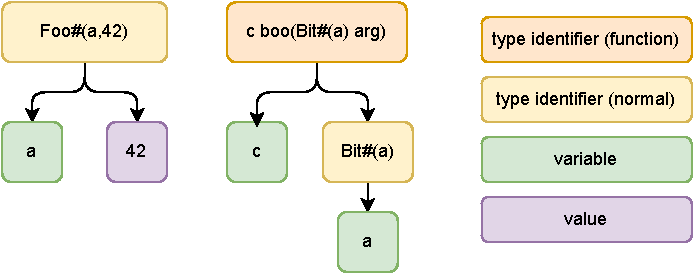
\includegraphics[width=0.7\columnwidth]{pdfExports/LargeMap-FunctionBreakDown.drawio.pdf}
\end{figure}
\newpage
\par
In my code there are 4 main functions that combined allow for type resolution:
\begin{itemize}
    \item \verb!merge! function takes two type identifiers and returns dictionary (map) from names of variables to theirs values. It's similar to Prolog's unification operator.
    \item \verb!applyVariables! function takes a dictionary and a type identifier and returns a type identifier with all variables replaced by their values. This is more of a utility function.
    \item \verb!resolveTypeclass! function takes a type identifier that is an proposed instance of a typeclass and returns dictionary of learned variable values if proposed instance is a valid one otherwise it raises an exception. In Prolog terms this would be like looking which rule can be applied and returning resolved variables from applying that rule.
    \item \verb!solveProvisos! function takes a dictionary of variables and a list of provisos and returns a dictionary with variables learned by solving provisos or raises an exception if it's impossible to satisfy all the provisos. This is like checking predicates in Prolog.
    \item \verb!preprocessTypeclass! function that takes a typeclass and produces a look-up dictionary of typeclass instances for given group of names present in the instance of the typeclass.
    \item \verb!solveNumerical! function that takes list of size relationship provisos and returns dictionary of learned variables.
\end{itemize}
\subsubsection{How those functions can are used}
Using all of those functions, I can answer many questions like:
\begin{itemize}
    \item What known thing can be used as \emph{nth} argument of a given function ?
    \item Is it possible to call given function with given tuple of arguments ?
    \item What is the resulting type of function given certain arguments?
\end{itemize}
There are also more subtle uses of functions like \verb!merge!, for example, when I need to deduce exact types of members of certain interfaces.

\subsubsection{Merge function} 
This function works like two synchronized dfs's, that go through the trees (type identifiers) and apply logic based on nodes that are beginning currently visited. 
This function needs to account for quite a lot of special cases as each node can be one of the following: variable, value (integer), type identifier (normal), and type identifier (function). Fortunately, half of the cases are symmetrical to the other half. In broad strokes, here is the logic behind those cases: 
\begin{itemize} 
   \item If one of the nodes is a variable, and the other is a value or another type identifier, then we set the value of the variable to a value of the other. 
   \item If both nodes are values, we check if they are equal. 
   \item If both nodes are the same kind of type identifier, we recursively compare their children. (If there are not of a function kind, we also compare their names) 
   \item If both nodes are variables, then we need to check if it's possible to unify the values of those variables if so, we assign the value of those variables to the result of unification. 
   \item In other cases, like when we need to unify type identifier with value, we raise an exception. 
\end{itemize} 
One minor problem that I encountered was that I had to keep track of which variables are equal, but I was able to avoid this problem altogether using shared pointers. 
\subsubsection{Apply variables function} 
This function is quite simple. Simply recursively traverses a type identifier and replaces all variables with their values. 
\subsubsection{Preprocess typeclass function}
Earlier, I compared typeclass to groups of Prolog rules with the same name, one thing I did not mention is that typeclasses can also contain something called dependencies, they are something like marking inputs and outputs in Prolog. Those dependencies are used in typeclasses like \verb!Bits#(a,b)! which are used to determine something, and they make sure that the resolution of a typeclass is always unambiguous. \\ 
For example, typeclass \verb!Bits#(a,b)! has a dependency \verb!a determines b! which means that you can use it to determine \verb!b! from \verb!a!, but if you know only \verb!b! then you cannot use it to determine \verb!a! because there may be multiple types that can be packed to the bit vector of the same length \verb!b!. An example of determinable pair of \verb!a! and \verb!b! would be  \verb!a = Bit#(32)! from which we can determine that \verb!b = 32!. It is also worth mentioning that we can have multiple tuples of dependencies. For example, we can have typeclass \verb!Boo#(a,b,c,d)! with dependencies \verb!(a,b,d) determines c! and \verb!(a,d) determines (b,c)!. They mean that we need to know either variables \verb!(a,b,c)! or \verb!(a,d)!. From an implementation perspective, this is just extra complexity.   
\par  
Now, I observed that most typeclass instances use non-function type identifiers, so I can create a look-up dictionary for every tuple of names of type identifiers in the instance. This way I find a set of typeclass instances that can be used to resolve a typeclass. I also need to account for instances that have functioned as one of their parameters as this introduces nasty polymorphism and I decided simply to put those instances in a special group called universal instances that are always checked in the resolve typeclass function.  
\subsubsection{Resolve typeclass function}
This function in Prolog terms is like taking a predicate of a rule and then trying to check if it can be satisfied. This can be quite slow if there are many rules, but thanks to the lookup dictionary created during preprocessing. We can narrow down the set of rules to check. 
Then we can iterate over all typeclass instances (rules) and apply the following algorithm: 
\begin{enumerate}  
   \item Merge candidate instance with one  
   \item If merging succeeded, attempt to solve provisos. 
   \item If provisos were successfully solved, return the dictionary of resolved variables, otherwise continue iteration. 
   \item If all iterations have failed, fail. 
\end{enumerate} 
This procedure is a bit slow, so I speed it up by creating lookup dictionaries that take as a key a dictionary and as a value a typeclass instance. This method can cut down search time significantly, but there are still rules that use polymorphic functions, and those cannot be preprocessed away so easily. Therefore, I call them universal instances and search through them every time. While, I could invent many heuristics to speed up this process. In general, this is still as difficult as the halting problem. 

\subsubsection{Solve numerical function} 

This function takes a set of size relationship provisos and a dictionary of variables. Then it converts those provisos into a set of equations on natural numbers. If the set is unsolvable this function raises an exception. Solving is done using the SymPy library. 
From an implementation standpoint, I just need to traverse the tree of type identifier describing proviso and for each \hyperref[sec:Provisos]{name of proviso} TODO (check this) I convert it into a mathematical expression. Exact expressions were taken from the Bluespec reference manual. 
\subsubsection{Solve provisos function} 
As established earlier, provisos can be of two types, one is based on typeclasses and those can be resolved using \verb!resolveTypeclass!, and the other ones are size-based and require solving sets of equations on integers and this can be done using \verb!solveNumerical! function. 
One big problem is the lack of order in which provisos must be solved. Therefore, I handle this by creating a set of provisos to be solved. Then I repeatedly iterate over this set and remove solved provisos. If the set does not change after iteration, and it is not empty this means no further progress can be made, and the function raises an exception. 


\newpage

\section{Synthesizing the module}
This is probably the simplest part of the project. I just iterate over various kinds of things defined by the user and run some string formatting code. Even for busses, thanks to polymorphism in the Bluespec I can quite easily write a routing function. 
  
  
The main goal of the project is to be able to take a JSON with some data and synthesize a top module in the Bluespec language from it. This goal is more like a justification to create a language server like API. With this approach, I have some simple core goals, but in the later sections, we will see how thanks to all the work I have done, this API can be used to support a GUI that aids the user in creating a top module. Therefore, I will focus in this section on how the API works, and only later, on how is it used when reading JSON or as a backend to the GUI based app. 
  
  
\subsection{JSON interface}
I decided that my \say{human-readable format} will be JSON. This format is simple, and support built-in in many languages.
The only problem with JSON is that it is more verbose than in some aspects Bluespec, and in theory, it would make more sense to use Bluespec.
However, this could introduce user confusion, as I am not able to support arbitrary Bluespec features in my backend.
My understanding is that supporting something only partially could lead users to think that my tool is broken because it does not match their assumptions about what it can do.
While it can be argued that if I had written this project as an extension of the Bluespec compiler, I could have supported all features of Bluespec (thanks to already written logic in the compiler).
I explained, at the beginning of this document, why doing this was infeasible for me as a part II project.
At the same time, using JSON allows me to support simplified semantics for things like bus creation and features not found in Bluespec like the specification of folders with additional libraries.

\newpage 

\subsubsection{Structure of JSON file}

\begin{figure}[h!]
    \centering
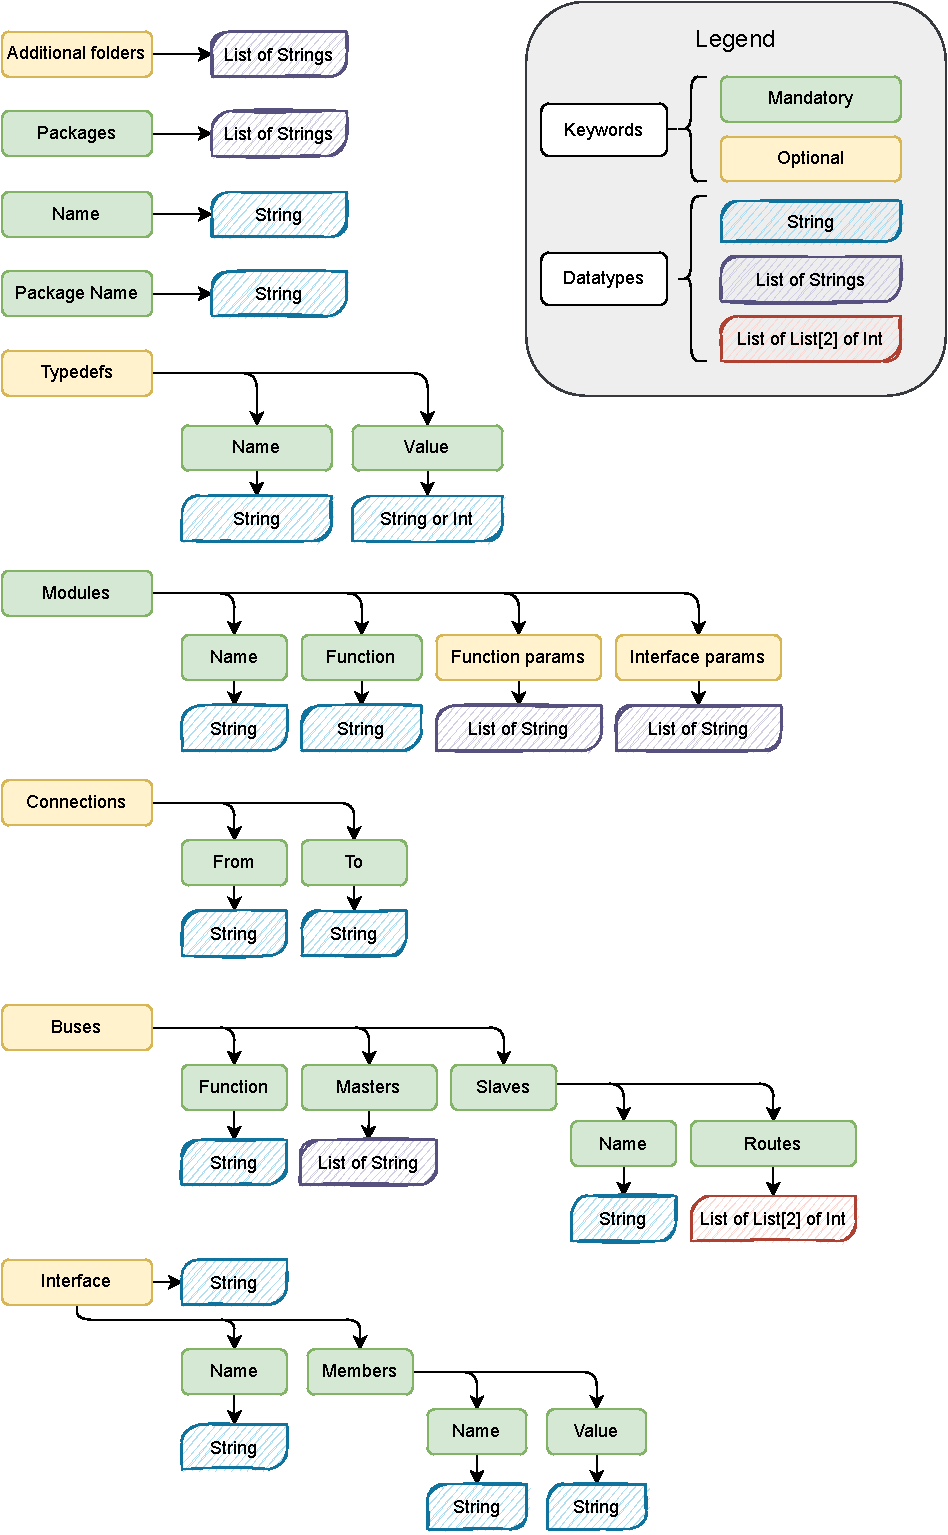
\includegraphics[width=0.70\columnwidth]{pdfExports/LargeMapJSON.pdf}

\caption{Disclaimer: In this diagram, I am using uppercase names but the JSON file uses lowercase ones also all spaces are replaced with underscores. I am also using s in the name to signify a list of dictionaries with those keywords}

\end{figure}
\newpage
More detailed description of keywords: 
\begin{itemize} 
   \item \verb!additional_folders! - list of folders that will be added to Bluetcl search path. 
   \item \verb!packages! - list of packages that will be used 
   \item \verb!name! - name of the module (defaults to \say{top}) 
   \item \verb!package_name! - name of created package 
   \item \verb!typedefs! - list of typedefs defined by a user 
   \item \verb!typedefs[i].name! - string starting with uppercase 
   \item \verb!typedefs[i].value! - integer or string (TODO check if string works) 
   \item \verb!modules! - list of modules or function to be instantiated 
   \item \verb!modules[i].name! - string being name of a module (used later to access such module) 
   \item \verb!modules[i].function! - lowercase name of a function used to create a module 
   \item \verb!modules[i].func_params! - list of strings that will be parsed, this can include numbers, names of interfaces of previously declared modules, \verb!tagged <Keyword>! where \verb!<Keyword>! can be replaced with struct creator. (TODO check if it works) This keyword is optional if function does not take any arguments. 
   \item \verb!modules[i].interface_params! - parameters passed to the interface of the result of the function, this keyword is optional if the full type of the interface can be inferred from the type of function used to create a module, arguments, and provisos. 
   \item \verb!connections! - list of dictionaries containing definitions of connections 
   \item \verb!connections[i].from! - lowercase string with access path of a left side of the connection 
   \item \verb!connections[i].to! - lowercase string with access path of a right side of the connection  
   \item \verb!busses! - list of dictionaries describing busses 
   \item \verb!busses[i].function! - lowercase name of a function used to create a bus 
   \item \verb!busses[i].masters! - list of access paths of interfaces to use as masters 
   \item \verb!busses[i].slaves! - list of dictionaries describing slaves 
   \item \verb!busses[i].slaves[j].name! - access path of an interface used as slave 
   \item \verb!busses[i].slaves[j].routes! - list of lists length two of integers describing starts and ends of address ranges on which slaves will be accessible. Starts of ranges are inclusive, and are exclusive. (This data is used to generate routing function) 
   \item \verb!interface! - either a string describing an access path of an interface to be exposed by a module or a dictionary describing a more complex interface made out of multiple member interfaces and methods 
   \item \verb!interface.name! - name of a type of the interface, if one is not present in loaded packages a new interface will be synthesized 
   \item \verb!interface.members! - list of members methods and subinterfaces of this interface 
   \item \verb!interface.members[i].name! - name at member will be accessible 
   \item \verb!interface.members[i].value! - access path of a method or an interface to be exposed at given name  
\end{itemize} 


\subsubsection{Using JSON interface}

If all I did was simply synthesize a Bluespec file describing a package from JSON, it would be mostly (one would need additional data to synthesize a new interface) possible to do that just by doing simple string manipulation.

I know this because my initial iterations were doing this. However, my tool can do much more than that. To show those abilities, I print additional data and verify the correctness of the given JSON. Below is a rundown of this additional data, but to truly appreciate it, I would recommend looking at how GUI is using this data.

\begin{itemize}
\item Dictionary of all possible connections, better interface and subinterface and methods of instantiated modules.
\item Dictionary of possible valid arguments for each function used to instantiate a module or a function. 
\item Dictionary of possible other masters and slaves for each instantiated bus.
\item Inferred types of every instantiated module and types it is subinterfaces and member methods.
\end{itemize} 

All this data can be useful when using complex modules from foreign packages, like a CPU core that does not have any direct connections, but has many subinterfaces that can be connected to things like memory, external devices, etc.

\section{GUI}
Adding GUI was an optional goal mentioned in the project proposal. I originally intended to use a game engine, but the Bluespec compiler is a Linux tool and game engines like Unreal Engine 4 or Unity3d are optimized to be used on Windows, so I decided against that idea. Instead, I found a library called React Flow, that provided a simple API for creating graph-based user interfaces. Therefore, I decided to create a GUI as a website. This was quite an adventure as It was effectively my first contact with web development. (I have done backend in .NET and \verb!C#! for a group project in the last term, but it was mostly focused on writing queries to database and I had no contact with frontend development)

\subsection{Backend}
For the backend, I had a choice between Django and Flask (as those are the main python libraries for backend development). After reading about them in theory, Flask was supposed to be better for small projects, like this one. However, I decided to use Django because I wanted to learn techniques that will be more useful in the future. I followed an official tutorial on Django and after initial pain with security, adding new functionality was easy.

\subsection{Frontend (React)}

The frontend was written in React.js as you might have guessed from the name of the library I wanted to use. According to \href{https://insights.stackoverflow.com/survey/2021#most-popular-technologies-webframe}{Stack Overflow 2021 survey}, React.js is the most popular frontend technology in 2021, so again I considered time spent on learning it to be a worthwhile investment. One thing that took me quite a bit to get used to is everything being a function (React.js supports classes, but it is an old paradigm and I wanted to learn to do things the \say{correct} way). This makes working with variables a bit tricky, as changes to state variables cause re-rendering of the whole component, and if a variable is not a state variable, then its value is going to be lost after re-rendering. If not careful, it is easy to cause a feedback loop causing infinite re-rendering and subsequent crash of the application.
\subsection{Frontend (React Flow)}

\begin{tcolorbox}[title=Vocabulary]

\begin{itemize}

\item Handle - Is a component of node that is used to start or end a connection. TODO include an image of a handle.

\end{itemize}
\end{tcolorbox}
React Flow from a developer perspective requires defining nodes (they can be arbitrary React components), and some metadata about displaying a graph that is things like how edges look, how a user can add new nodes, etc. 
The exposed API is quite simplistic. 
For example, the position of a handle is constrained to the middle of the side of a node, and this library will generate CSS to put it there. 
Therefore, I needed to write some finicky CSS to align the handle with text displaying its name. [TODO improves this sentence.]
\\
Another thing that is problematic about React Flow is that it will cause the node component to update every time it is moved.
What I found is that if you wrap larger subcomponents of a node in \verb!memo! from React, then performance stays quite good even if multiple nodes are moving, as React will cache rendered subcomponents.
\\
On the bright side, after I figured out workarounds for those issues, I was left with many other things being handled by the library. This included automatic graph formatting and pretty Bézier curves for edges. 

\subsection{Frontend (MUI)}

Default HTML buttons and text boxes are ugly. So, I decided to use React UI component library called MUI (previously Material UI). I do not have much to say about it except that use of it was frictionless, at least in my humble opinion it made my application look modern. I am mentioning this as one of my complaints about Intel's platform designer was that its UI is decades old.
 
\subsection{Functionality} 
After teasing how I did things, let us talk about the features of my GUI.  
Using this GUI, a user can do the following things.  
\begin{itemize} 
   \item Instantiate new module.  
   \item Connect two interfaces. 
   \item Create a bus. 
   \item Select methods and interfaces to be exported as a part of a created module. 
   \item Look at created Bluespec file. 
   \item Run compilation followed simulation and look at the output of both.  
\end{itemize} 
To do all those things, the user will need to interact with the graph building tool. Below is an overview of components users can choose from that will describe the top-level module. 
\subsubsection{Instance node} 
This node is most important as using it the user can instantiate new modules, convert between interfaces, and use functions in general. It can be in 3 main stages. During the first one, it is an empty vessel, using which one can specify its name and function/module that will be used. In the second stage, a user specifies inputs and typing information. Finally, after clicking \emph{confirm update} node transitions into stage three and interfaces and methods of a created object become usable. 
\newpage 
\begin{figure}[!h] 
   \centering 
    
   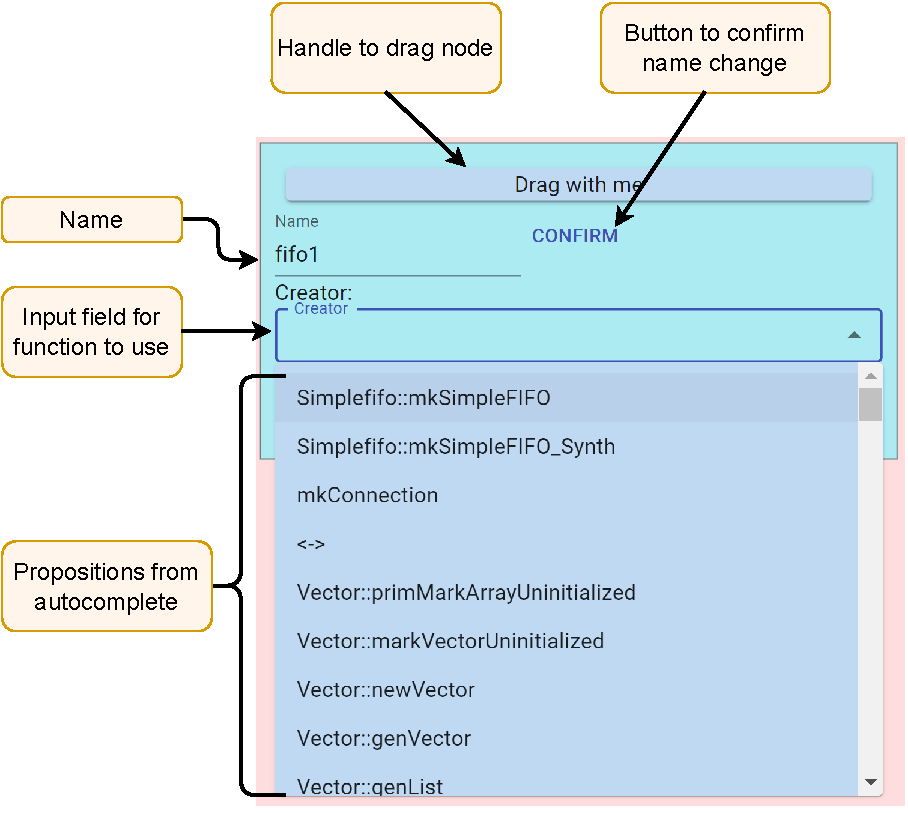
\includegraphics[width=0.63\columnwidth]{pdfExports/LargeMapInstanceNode.pdf} 
   \caption{Stage one of node used to instantiate new modules} 
\end{figure} 
At stage one we will see the first field with autocompletion, it is the simplest one and simply lists all functions/modules user can use. It contains stand-alone functions as well as functions found as part of typeclasses. A node will transition to stage two when one of those is picked. 
\begin{figure}[!h] 
   \ centring 
    
   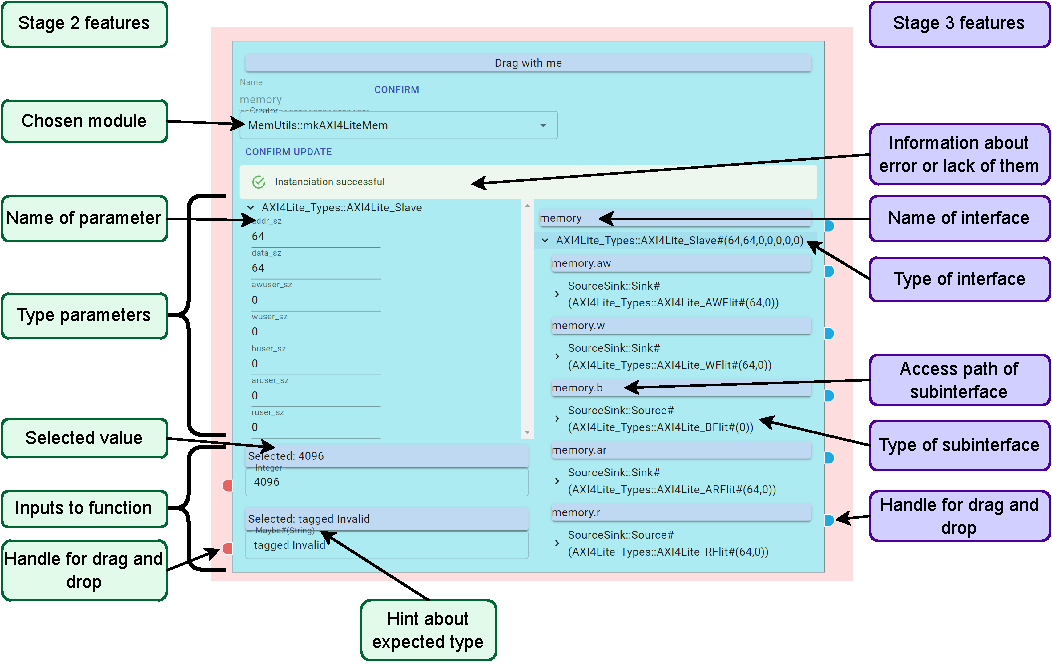
\includegraphics[width=1\columnwidth]{pdfExports/LargeMap-InstanceNodePart2.drawio.pdf} 
   \caption{Fully instantiated node with descriptions of features, divided into stages two and three} 
\end{figure} 
At stage two, the user can specify typing information. To do this, they are presented with a tree-like input structure. Values inputted there can be of either uppercase string describing type identifier, integers or lowercase strings that will be used as a variable that is meant to be resolved by the backend. There is also a list of inputs that go directly to the function. Those inputs contain fields with autocomplete that will filter all typedefs found in loaded packages, interfaces and functions found in previously initialized nodes. Some handles allow for the drag and drop style of creating connections. If the user chooses a value via a text field that is a member of a previously initialized node, then the connection will be generated automatically. 
After a user is satisfied with their choices, they press the \emph{confirm update} button. 
At stage three, the user is presented \emph{information about the error or lack of such} this can take bar can be in one of three states, its functionality is shared between nodes. 
\begin{itemize} 
   \item Waiting for confirmation - When the backend is processing data. 
   \item Instantiation successful - If everything went smoothly. 
   \item Error with text that tries to describe and error that occurred. This usually occurs after the user-supplied data is not able to satisfy the provisos of a function used. 
\end{itemize}  
In case of lack of errors, a user is given an overview of the interface of the object created with its subinterfaces and methods and their types. Attached to them are handles for starting connecting using DnD. 
\newpage
\subsubsection{Connection node}
\begin{figure}[!h]
\centering
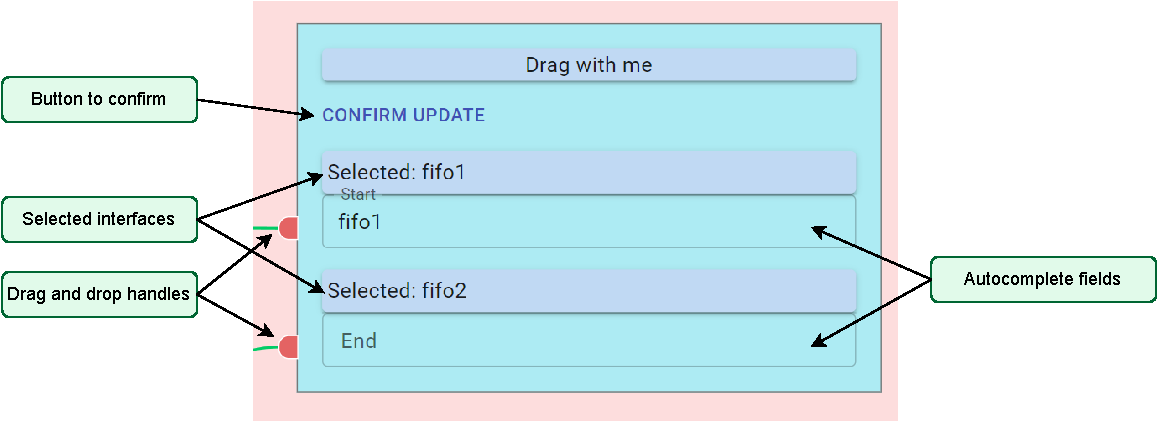
\includegraphics[width=1\columnwidth]{pdfExports/LargeMap-ConnectionNode.drawio.pdf}
\caption{Connection node, connecting two FIFO modules}
\end{figure}
This is the simplest node, it contains two inputs, like the ones found in the instance node. The key change hides in autocompletion, \emph{start} field will show all modules that can be used to start a connection, whereas \emph{end} will only autocomplete the things that can be connected to the thing specified in the start field. The power of this node lies in the fact that it uses typing information in the backend, and it will work with new any types if there is an applicable instance of typeclass \verb!Connectable! which should be common as it is part of the standard libraries.

\subsubsection{Bus node}
\label{sec:AutocompletionBusNode}
\begin{figure}[!h]
\centering
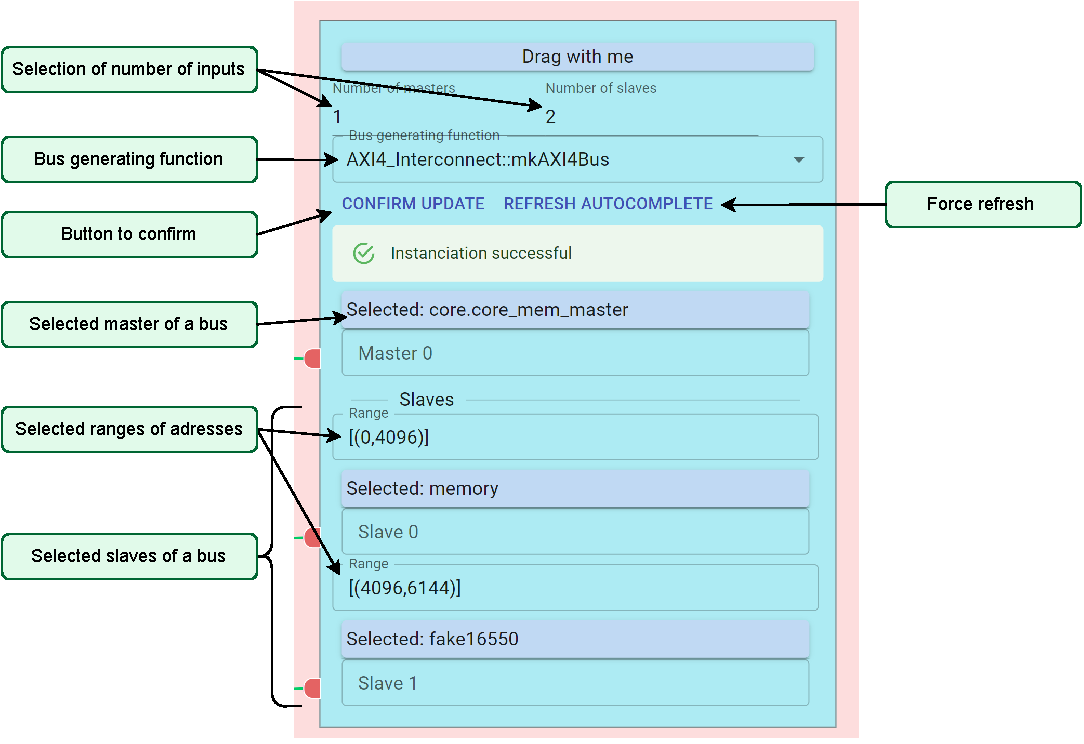
\includegraphics[width=1\columnwidth]{pdfExports/LargeMap-BusNode.drawio.pdf}
\caption{Bus node connecting one master and two slaves using AXI4 interface}
\end{figure}

Similarly to the connection node, most of the components were reused, and interesting are the details. This node works only with a subset of functions, that have specific something (TODO find a word to use). Fortunately, used do not need to look for those functions, autocomplete field will only show you valid ones. (It might be possible that some non-bus function will slip through as I do not want to be overly aggressive and require things like having \say{bus} in the name of the function, but from my testing, my simple check narrows down options to less than ten from few thousand found in all packages, I worked with.).

Autocompletion for masters and slaves is a bit more nuanced, as it has two levels of precision. At the first level, it will show all masters and slaves that can be used with chosen function, but not necessarily together. However, after the first successful initialization of a node (using \emph{confirm update}), options for masters and slaves will be narrowed down to only ones that can work with masters and slaves selected during the first initialization.
This node also contains fields to select ranges of addresses on which slaves will be visible. 
\newpage
\subsubsection{Exported interface node}
\begin{figure}[h!]
\centering

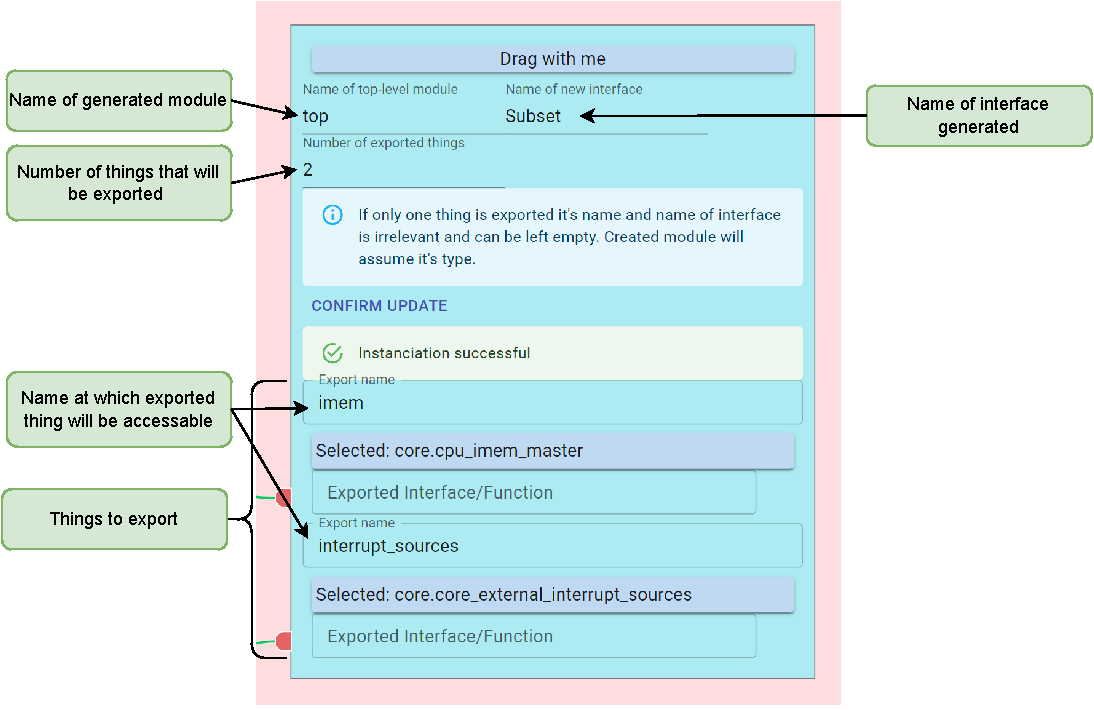
\includegraphics[width=0.8\columnwidth]{pdfExports/LargeMap-ExportNode.drawio.pdf}
\caption{Overview of features of a node, allowing to export things from a created module}
\end{figure}
This node allows users to specify the name of a function creating a module they designed. Name of the interface which will be used by this module if it will need to export more than one thing, and most importantly, all the exported interfaces. If a name of an interface is already known, the system will try to populate members of that interface with members provided, if the name is not known it will simply create a new interface using all the typing data from the members. It also contains a simple feature which will generate a name based on the access path if the user will not provide one. 
\par
The intention behind this node is that one might want to create their system partially in Bluespec and partially in Verilog, as there are vast libraries of IP written in Verilog. Using this node one can create a new interface on a fly that does not have much use in Bluespec world, but if transpiled to Verilog it will only contain things user-specified, making the process of importing it into tools like Platform Designer much easier. 
\begin{tcolorbox}[title=Futher work (TODO this can be removed)]It's worth keeping in mind that for a GUI like this, there is a multitude of things that can be added. Here is a list of things that could be added: 
\begin{itemize}
\item Ability to add comments that partition the graph (like in UE4).
\item Inputs' node to be able to select inputs to a module. Therefore, allowing for parametrization.
\end{itemize}
\end{tcolorbox}

\chapter{Evaluation}
Throughout working on this project I have learned a lot about QSys and Bluespec, and how they interact. This means that I will need to adjust slightly it from the project proposal to better represent problems that are solved. Firstly my understanding is that Platform Designer tool is shared between QSys and QSys Pro.

\section{Overview}
My evaluation will be divided into three examples:
\begin{itemize}
    \item First one will be about connecting FIFOs.
    \item Second will show a simple system-on-chip (SOC). With one Flute core, memory module and fake interface with outside world, all connected by a bus.
    \item Third example will two AXI4 masters and two AXI4 slaves connected by a bus. 
\end{itemize}
First two examples will produce valid devices, but they won't do anything interesting. Last example will produce a working top level module that will demonstrate that generated code indeed produces same results as connection modules using Platform designer.

\subsection{Polymorphism disclaimer}
Before we start talking about examples we need to address the elephant in the room. There is no support for Bluespec in IQP (nor Xilinx Vivado). This means that when working with Bluespec and those tools, one must first transpile Bluespec to Verilog. Unfortunately, Bluespec compiler can't generate Verilog code of functions that are polymorphic (TODO or take arguments TODO check this). This happens because typing system of Bluespec is much richer than one of Verilog. Therefore, any module used with IQP will need to be converted into it's synthesizable version stripped of any arguments before being transpiled into Verilog. One might argue that this is an issue with Bluespec and not with those tools, but I would argue that it is still a problem that needs fixing, and I have solution for It. 


\section{Example 1 - Connecting FIFOs}
In this example our goal is to create two connected FIFOs and then modify the system to connect a third one. FIFOs that I will be using have an interface analogue to the FIFO interface found in default Bluespec libraries. This way source code for them is self-contained within a simple file. This interface consists of following things: (Action and Value are types of methods, TODO maybe add types)
\begin{itemize}
    \item Action Enq - Available if queue is not full, it enqueues the data.
    \item Action Deq - Available if queue is not empty, then removes the first element.
    \item Value first - Available if queue is not empty,returns the value of the first element.
\end{itemize}
In Bluespec there are provisos attached to those functions, and if in given cycle user will want to perform illegal operation (like dequeue when queue is empty) then rule in which this operation would be performed simply won't fire in that cycle. In Verilog there is no notion of such provisos nor method, so everything needs to be synthesized with the aid of wires creating Ready-Enable micro protocol. Every method has Ready and Enable wires. When Ready is high, then method is allowed to be executed. When Enable is high, it signals to the device to execute given method.(TODO fix wording)
\subsection{Platform Designer}
To create a system with two connected FIFOs, we first need to import them into platform designer. Here we encounter first problems. As mentioned before, Bluespec can't generate Verilog code of functions that are polymorphic. So we must decide on the width of the data stored in such FIFO before transpiling to Verilog. After export of the Verilog file it needs to be imported into the Platform designer. This tool perfroms analysis of a file, which results in decision tha tall wires found are parts of Avalon slave interface. This is an obvious error, and we need to correct it by hand.
\begin{figure}[H]
    \centering
    
    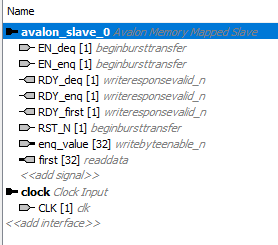
\includegraphics[width=0.5\columnwidth]{images/Example1BeforeOranization.png}
    \caption{Zoom in on the arrangement of wires after import}
    \end{figure}
This is unfortunately easier said than done. There are few options of assigning those wires, but neither of them perfect. Firstly we will need to choose a type of interface those will represent. In Platform designer we have over 30 options to chose from, but most of them are variants of complex protocols like AXI4. The only option that will make sense for us is \emph{Conduit}, which basically meaningless blank canvas. We could create a conduit for each method but after consultation with my supervisor he recommended creating a conduit for each wire. So I did as he recommended, and this produces following set of interfaces. This requires quite a bit of manual work, listed bellow.
\begin{itemize}
    \item Create 8 new interfaces (QSys figured out what to do with clock wire on its own, so we have one for free) this includes giving them a name and assigning a reset signal.
    \item More each wire to its respective interface and change signal type of each wire to something generic like wire from type given to it as part of Avalon slave interface. 
\end{itemize}

\begin{figure}[H]
    \caption{After assigning wires and Interfaces}
    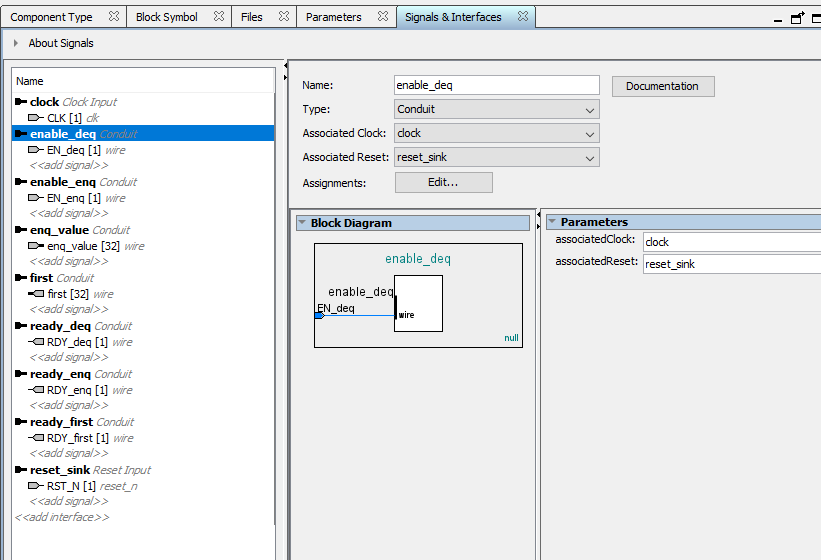
\includegraphics[width=\textwidth]{images/Example1AfterOrganization.png} \\
    \centering
\end{figure}

With all of those wires we can connect obvious things together like \verb!first! to \verb!enq_value! and clock signals, but then we run into a problem that with all wires that represent Ready-Enable micro protocol because we would like to enable enqueue in second queue only if both wires \verb!ready_deq! and \verb!ready_first! are high in the first queue, otherwise because we don't know how our FIFO is implemented we might run into a problem where we might get bugs(for example we lose data because we \verb!ready_deq! became high cycle faster than \verb!ready_first!, or in opposite scenario we would read stale/corrupted data). Unfortunately we can't create such logic using platform designer and one way of solving this would be to create special connector module that would do this logic(I'm going to come back later to this to explain why this approach might be infeasible in general case). 

\subsection{My tool}
Using my tool whole phase of importing and setting up wires can be skipped, as all data information needed is grabbed directly from packages. Connecting FIFOs is as simple as creating a new node connection node and selecting chosen FIFO's interface. Extending two connected FIFOs to three is as simple as adding one more FIFO and one more connection node.

\begin{figure}
    \caption{Three connected FIFOs using my tool (TODO update this graphic)}
    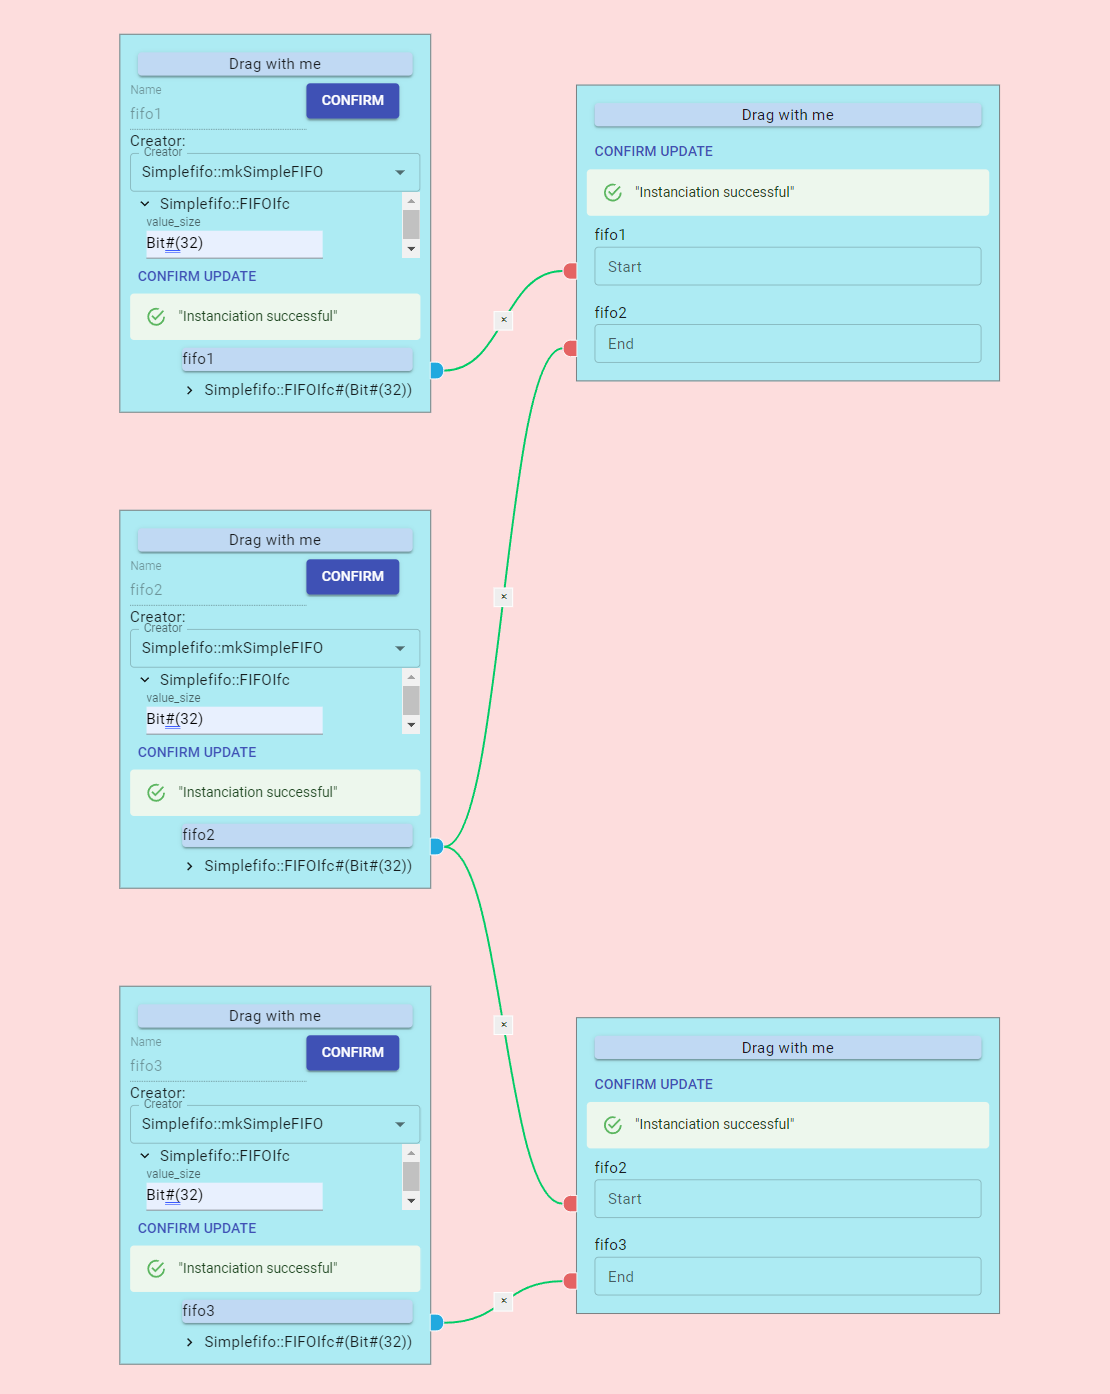
\includegraphics[width=0.7\textwidth]{images/Example1MySolution.png} \\
    \centering
\end{figure}

\subsection{Using text format to do same things and Qualitative metrics}
To count number of tokens I'm using following regexp \verb!(\w|\.)+!. This regexp will match sequences of alphanumerical characters with dots and underscores. (TODO draw graphs)
Raw numbers: 431 tokens to import FIFO, 347 for two connected FIFOs, and 415 for three connected FIFOs.
My solution: 31 for two connected FIFOs and 43 for three connected FIFOs.
\newpage
\section{Example 2 - Simple System-on-Chip}
In this example we will create a simple system-on-chip (SOC) with one Flute core, memory module and fake interface with outside world, all connected by a bus. This example is designed to even out playing field as all connections are done using AXI4 interface which is understood by platform designer.

\subsection{Platform Designer}
Again, we start with importing our modules. 
This time we need to import two of them, one for fake 16550 interface and one for flute core. 
As for memory module we will use one from IQP library to save time and effort.

Unfortunately platform designer can't figure out how to organize wires into interfaces like AXI4 master or AXI4 slave. 
So we need to do it manually. This wouldn't be so painful if not for the fact that we need to set type of each wire according to it's use. Fortunetly Bluespec compiler named them nicely, for example \verb!cpu_imem_master_awready! has type \verb!awready!. Each of those AXI4 interfaces has 37 wires, and if we account for all other interfaces of Flute core we get 150 wires that individually need to be assigned to interfaces. Similarly, our fake 16550 interfaces also uses 40 wires in total. When assigning this through GUI it took me around 16 minutes to roughly 80 wires that make up one AXI4 master and one AXI4 slave interfaces on the Flute-core and the Fake-16550. (For context tools like Xilinx Vivado have heuristics that are able to do a lot of this automatically, but my understanding is that it still only works for selected known interfaces)
\\
\begin{figure}[H]
    \caption{Connected Sys-on-Chip using Platform designer}
    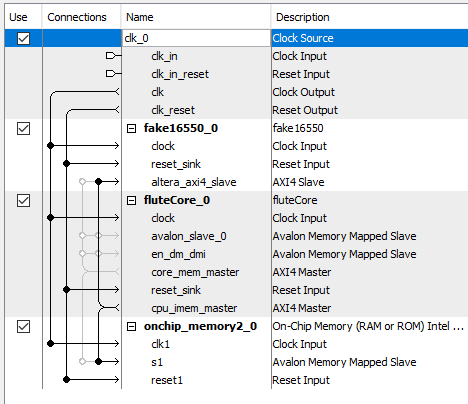
\includegraphics[width=0.7\textwidth]{images/Example2QSys.png} \\
    \centering
\end{figure}
After initial pain of importing modules we arrive at the point where Platform designer shines. It is able to show possible connections between AXI4 masters and slaves, on a 2D-grid-like layout. Connecting two together is as simple as clicking cross-section of two wires on the screen.  

\subsection{My tool}
Again using my tool we don't need to do anything to import modules, as all the typing information is provided by the package. To connect those together we create a special bus node, select function for creating a bus, select number of masters and slaves, then assign each accordingly. While I'm unable to show nice 2D-grid of possible connections, I have \hyperref[sec:AutocompletionBusNode]{two-stage autocompletion}.

\begin{figure}[H]
    \caption{Connected Sys-on-Chip using my tool(TODO update this image)}
    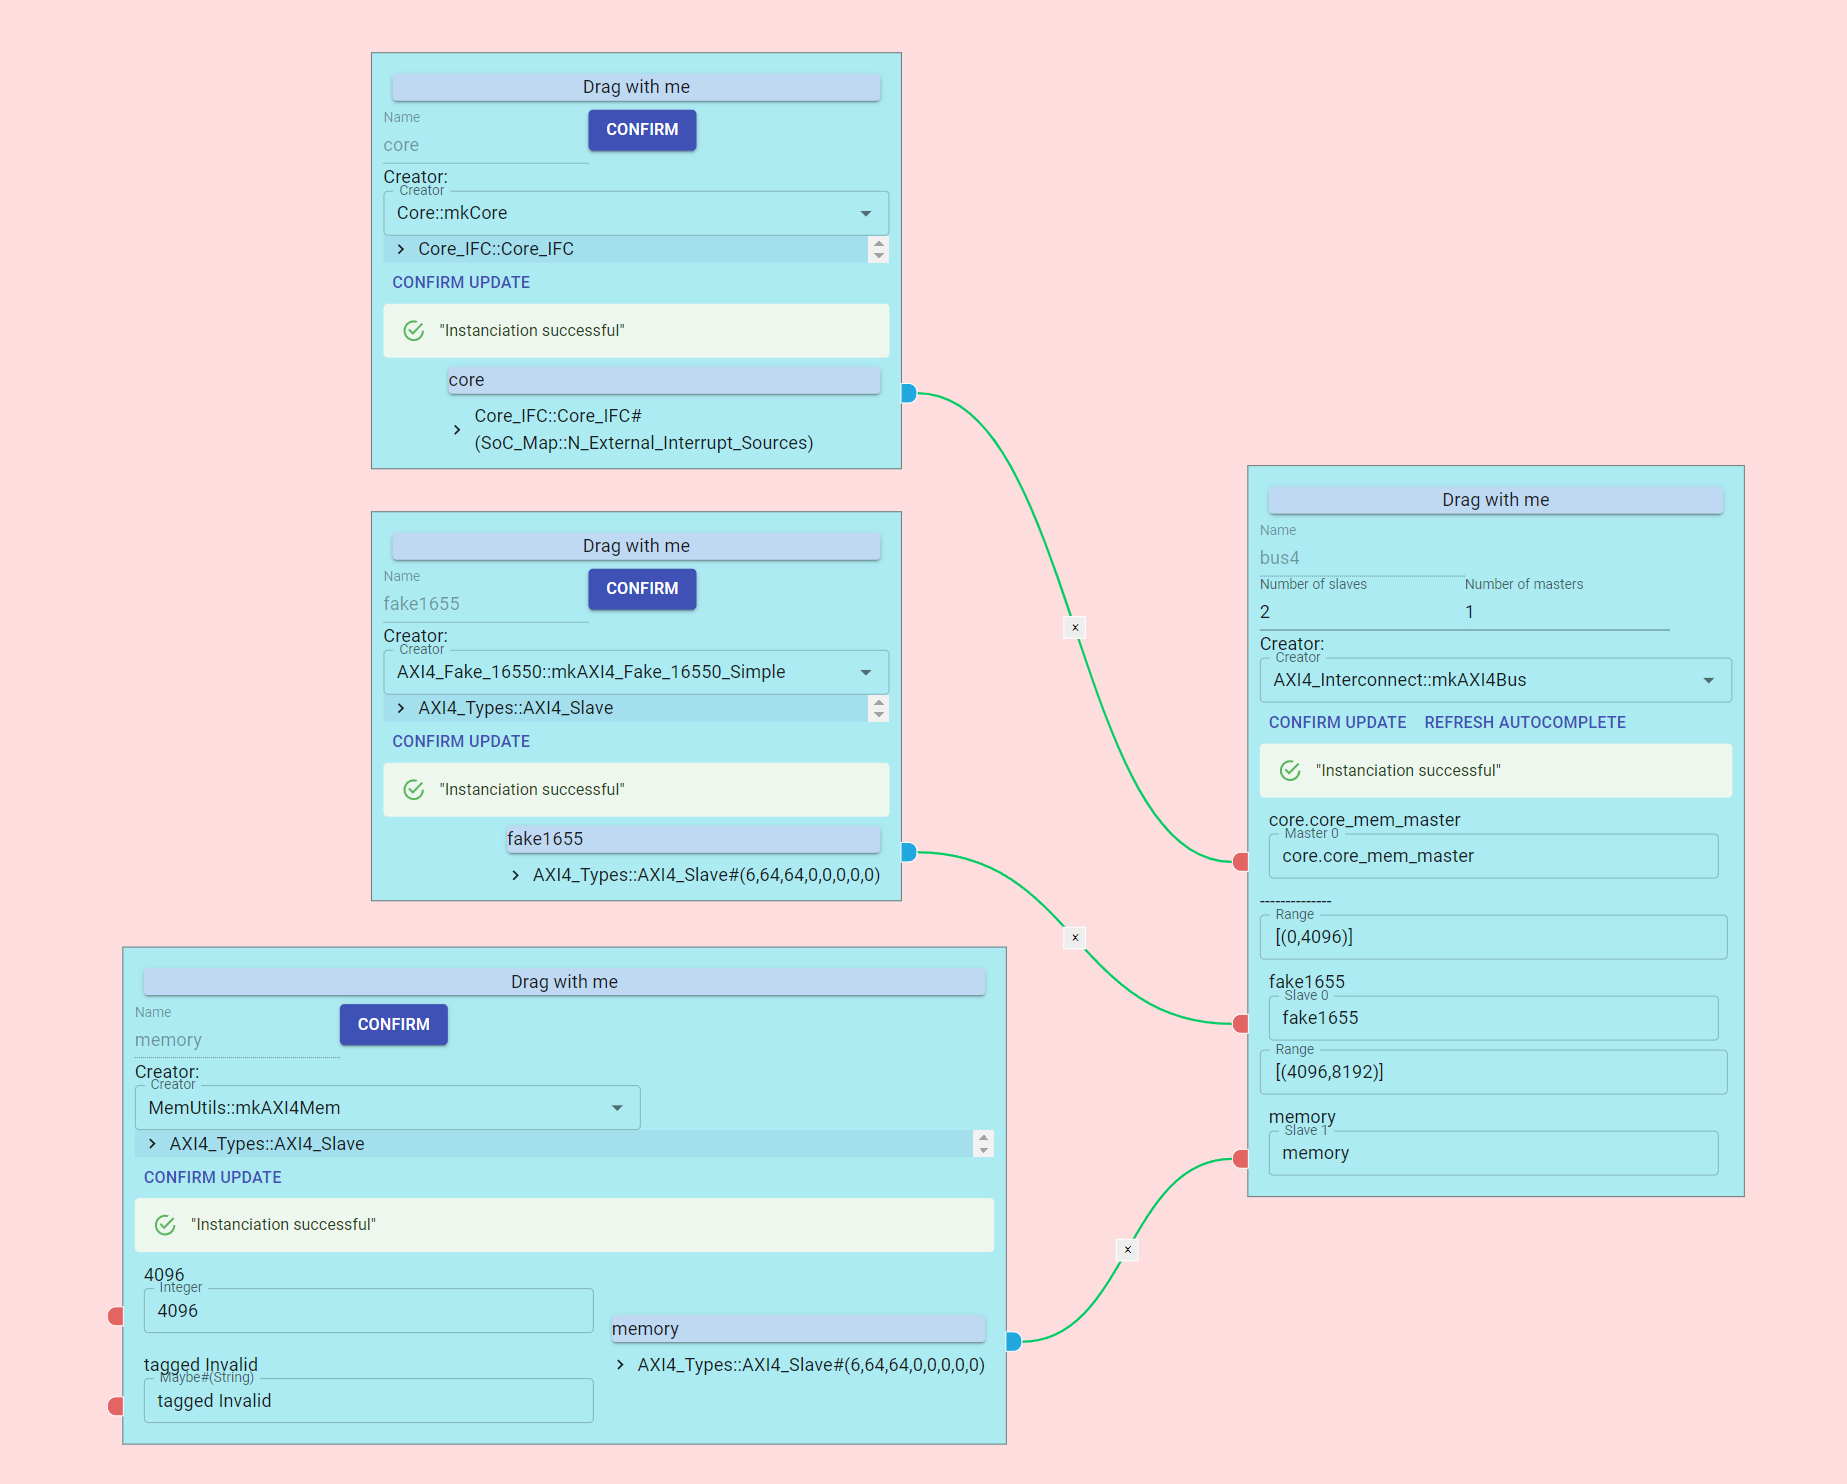
\includegraphics[width=0.8\textwidth]{images/Example2MySolution.png}
    \centering
\end{figure}

\subsection{Other differences}
There is a number of subtle differences that are worth talking about, but were not pronounced by this example.
\\
Platform designer has ability to automatically convert between AXI4 interfaces and Avalon ones, and also within those families it allows for some degree of flexibility when parameters don't match exactly.
When I create busses I'm limited by typing system, and way functions for creating buses were defined. Therefore, if user wants to do similar conversions they would need to use functions and perform those conversions by themselves(this would be node by inserting an instance node that uses function that does this convesion). 
\\
Another slight difference is the fact that in Platform designer, each master has its own bus, and while slaves can be connected to any number of masters they need to be connected individually. 
\section{Example 3 - Working AXI4 masters and slaves}
This example 

\section{Numbers}
\begin{figure}[H]
    \caption{Tokens used by each system for each example}
    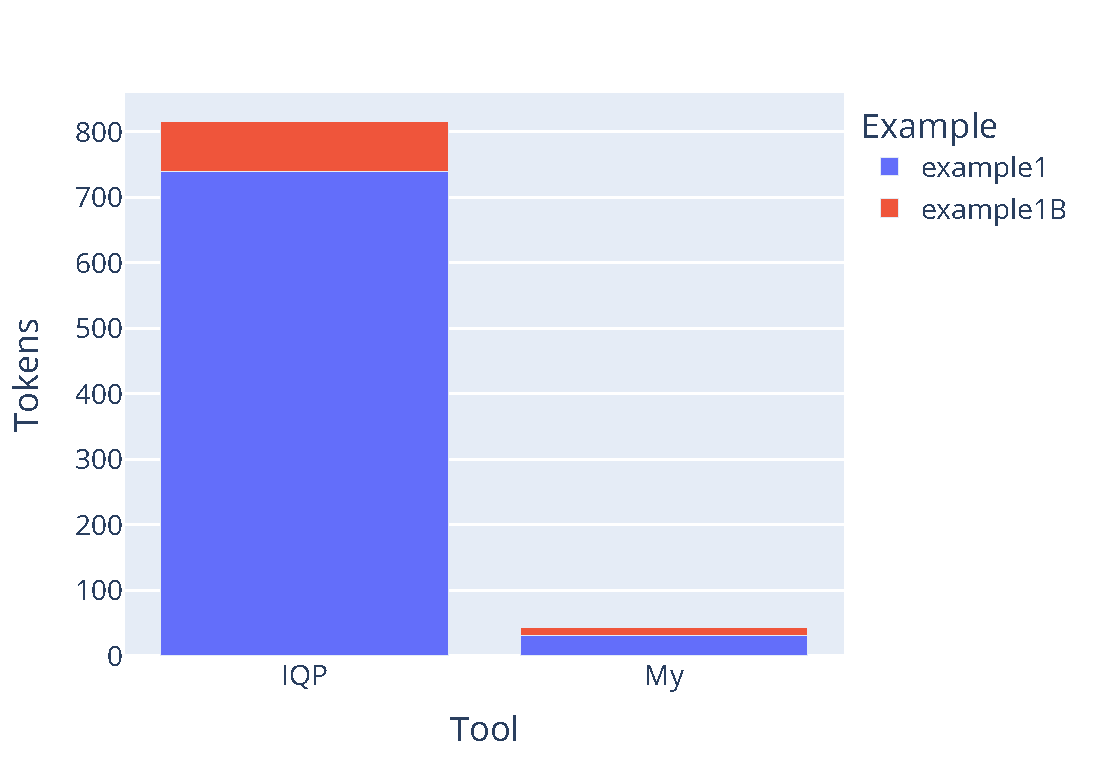
\includegraphics[width=0.8\textwidth]{charts/example1_tokens.pdf}
    \centering
\end{figure}
\begin{figure}[H]
    \caption{Lines used by each system for each example}
    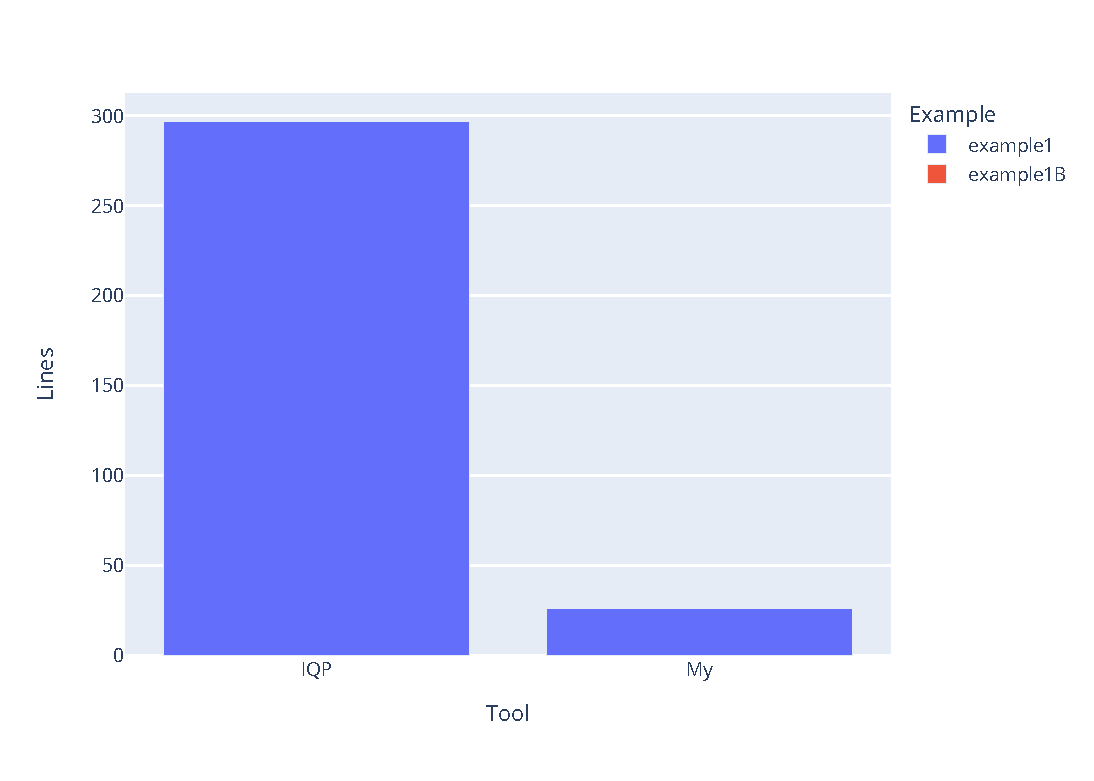
\includegraphics[width=0.8\textwidth]{charts/example1_lines.pdf}
    \centering
\end{figure}
\begin{figure}[H]
    \caption{Tokens used by each system for each example}
    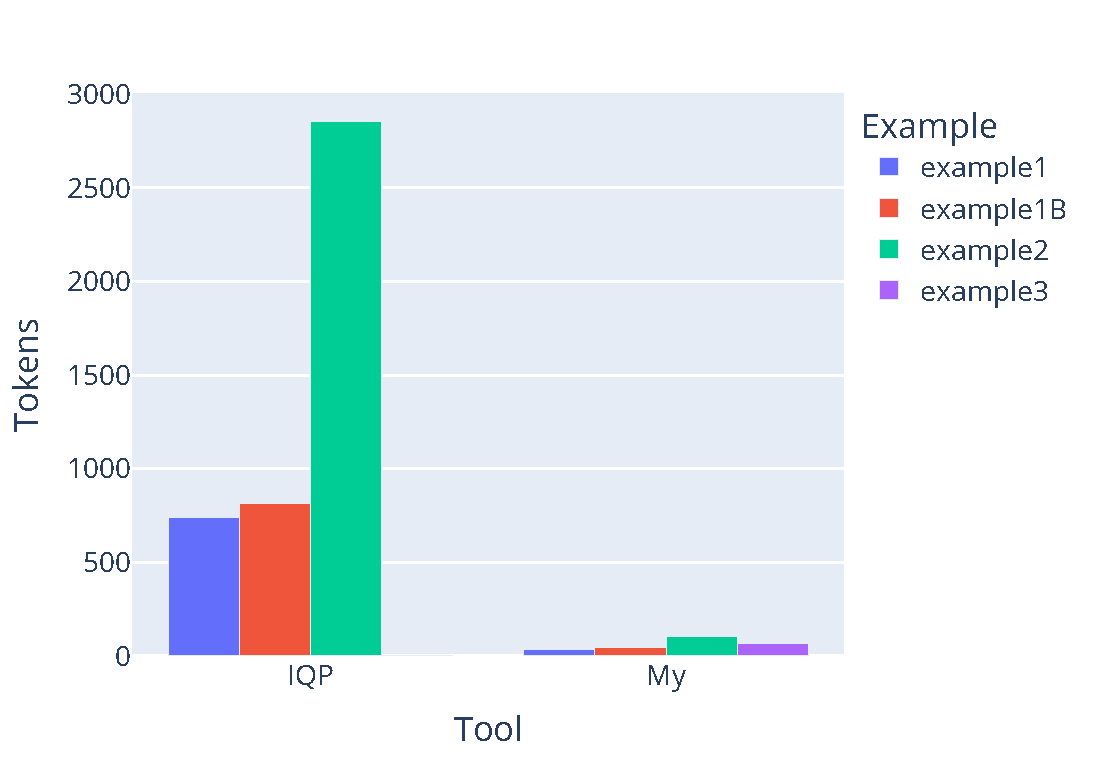
\includegraphics[width=0.8\textwidth]{charts/all_tokens.pdf}
    \centering
\end{figure}
\begin{figure}[H]
    \caption{Lines used by each system for each example}
    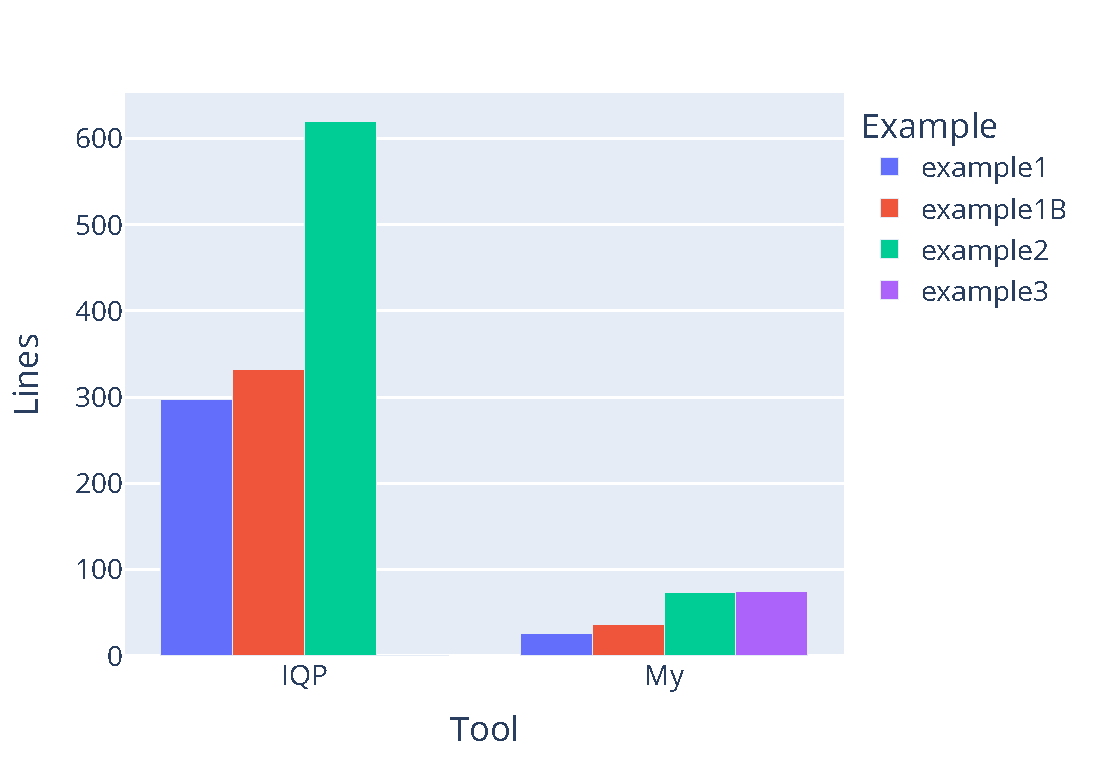
\includegraphics[width=0.8\textwidth]{charts/all_lines.pdf}
    \centering
\end{figure}

\chapter{Conclusion}
\section{Results}
I hope that I demonstrated how it can be used to speed up prototyping of high level modules in Bluespec. It's able to provide same basic functionally of allowing for connection and easy creation of busses as comparable tool made by intel. At the same time thanks to being Bluespec native it can drastically cut down time needed to import modules, especially if in cases where one wants to use polymorphic modules. While my tool isn't commercial grade, thanks to easy ability to synthesize exported interface, it allows for a workflow where everything Bluespec native can be connected using it, and then this part of a system can be imported to tool like Platform designer for connection to modules not available as a Bluespec library and connection of wires I/O on the FPGA.
\end{document}
